\documentclass{book}
\usepackage{graphicx}
\usepackage[english]{babel}
\usepackage{amsthm}
\usepackage{amssymb}
\usepackage{amsfonts}
\usepackage{mdframed}
\usepackage{physics}
\usepackage{tikz}
\usepackage[a4paper, margin=1in]{geometry}
\geometry{a4paper, margin=1in}
\usepackage{xcolor}
\usetikzlibrary{arrows.meta}
\usetikzlibrary{angles,quotes}
\graphicspath{ {./images/} }
\usepackage{svg}
\usepackage{stackengine}
\usepackage{subcaption}
\usepackage{bm}
\usepackage{empheq}
\usepackage{cancel}
\usetikzlibrary{decorations.text}
\usepackage[most]{tcolorbox}
\usepackage{tensor}
%3D
\usepackage{mathtools}
\usepackage{booktabs}
\usepackage{array}
\newcolumntype{C}{>{$}c<{$}}
\usepackage{tikz-3dplot}
\usepackage{appendix}
\usepackage{pgfplots}
\usetikzlibrary{shapes.geometric}
\usetikzlibrary{calc,patterns,angles,quotes}
%Tikz Library
\usetikzlibrary{angles, quotes, intersections}
\usepackage[bb=dsserif]{mathalpha}
\usetikzlibrary{decorations.pathmorphing}
\usetikzlibrary {patterns,patterns.meta} 
\tikzset{snake it/.style={decorate, decoration=snake}}

\usepackage{etoolbox} % ifthen
\usepackage[outline]{contour} % glow around text
\usetikzlibrary{calc} % for adding up coordinates
\usetikzlibrary{decorations.markings,decorations.pathmorphing}
\usetikzlibrary{angles,quotes} % for pic (angle labels)
\usetikzlibrary{arrows.meta} % for arrow size
\usepackage{xfp} % higher precision (16 digits?)

\usepackage{tcolorbox}

%https://osl.ugr.es/CTAN/macros/latex/contrib/tcolorbox/tcolorbox.pdf
\tcbuselibrary{breakable}
\tcbset{%any default parameters
	width=0.7\textwidth,
	halign=justify,
	center,
	breakable,
	colback=white    
}

\newenvironment{aside}
{\begin{mdframed}[style=0,%
		leftline=false,rightline=false,leftmargin=2em,rightmargin=2em,%
		innerleftmargin=0pt,innerrightmargin=0pt,linewidth=0.75pt,%
		skipabove=7pt,skipbelow=7pt]\small}
	{\end{mdframed}}

\renewcommand{\cleardoublepage}{\clearpage}

\usepackage[outline]{contour} % glow around text
\usepackage{physics}
\usepackage{xcolor}
\usepackage{etoolbox} %ifthen
\usetikzlibrary{calc}
\usetikzlibrary{arrows,arrows.meta}
\usetikzlibrary{decorations.markings}
\usetikzlibrary{angles,quotes} % for pic (angle labels)
\usetikzlibrary{fadings}
\tikzset{>=latex} % for LaTeX arrow head
\contourlength{1.4pt}

\colorlet{wall}{blue!30!black}
\colorlet{myblue}{blue!70!black}
\colorlet{myred}{red!70!black}
\colorlet{mydarkred}{red!50!black}
\colorlet{mylightgreen}{green!60!black!70}
\colorlet{mygreen}{green!60!black}
\colorlet{myredgrey}{red!50!black!80}
\colorlet{myshadow}{blue!30!black!90}
\tikzstyle{wave}=[myblue,thick]
\tikzstyle{mydashed}=[black!70,dashed,thin]
\tikzstyle{mymeas}=[{Latex[length=3,width=2]}-{Latex[length=3,width=2]},thin]
\tikzstyle{mysmallarr}=[-{Latex[length=3,width=2]}]
\usetikzlibrary{decorations.text}

\newcommand\rightAngle[4]{
	\pgfmathanglebetweenpoints{\pgfpointanchor{#2}{center}}{\pgfpointanchor{#3}{center}}
	\coordinate (tmpRA) at ($(#2)+(\pgfmathresult+45:#4)$);
	\draw[white,line width=0.6] ($(#2)!(tmpRA)!(#1)$) -- (tmpRA) -- ($(#2)!(tmpRA)!(#3)$);
	\draw[mydarkred] ($(#2)!(tmpRA)!(#1)$) -- (tmpRA) -- ($(#2)!(tmpRA)!(#3)$);
}
\newcommand\lineend[2]{
	\def\w{0.1} \def\c{30}
	\draw[mygreen] (#1)++(#2:\w) to[out=#2-180-\c,in=#2+\c] (#1)
	to[out=#2+\c-180,in=#2-\c]++ (#2-180:\w);
}
\def\tick#1#2{\draw[thick] (#1) ++ (#2:0.1) --++ (#2-180:0.2)}

% INTERFERENCE FADING
\begin{tikzfadingfrompicture}[name=interference]
	\def\lambd{0.5} % wavelength
	\foreach \r in {1,...,15}
	\foreach \j in {1,...,25}
	\path [line width=\lambd*\j,draw=transparent!0,opacity=0.04]
	(0,0) circle (\lambd*\r); %(0:\r) arc (0:180:\r);
\end{tikzfadingfrompicture}

\title{Electromagnetism 2}
\author{Dominik Szablonski}
\newtheorem{law}{Law}
\newtheorem{klaw}{Law}
\newtheorem*{definition}{Definition}
\newtheorem*{theorem}{Theorem}

\pgfplotsset{compat=1.18}
\begin{document}
\maketitle

\tableofcontents

\chapter{Sources of Radiation}
Radiation is the phenomenon of energy being transported to an observer. Radiation must be disconnected from its source. Plane electromagnetic waves satisfy conditions of being radiation, and are thus known as free fields. The source of electromagnetic radiation must be charges as those generate the electric and magnetic fields. However, electromagnetic radiation is only generated through accelerating charges. For a free field, there must be locations where radiation propagates while $\rho = 0$.
\section{Charges}
\subsection{Stationary Charges}
For a stationary charge, we can write,
\begin{align}
	\vb{E} = \frac{1}{4\pi\varepsilon_0}\frac{q(\vb{r} - \vb{r}')}{|\vb{r} - \vb{r}'|^3} \propto \frac{1}{|\vb{r} - \vb{r}'|^2} && \vb{B} & = 0
\end{align}
We can clearly see that a stationary charge cannot radiate as it has no component in $\vb{b}$. Furthermore, the energy flow varies as $\vb{1}{r^2}$, which require $\vb{E}\propto\frac{1}{r}$ and $\vb{B}\propto\frac{1}{r}$ which neither field satisfies.
\subsection{Charges with Uniform Velocity}
We can perform a Lorentz boost in the case of a moving charge,
\begin{equation}
	\vb{E}(\vb{r}) = \frac{q}{4\pi \varepsilon_0}\frac{1-\beta^2}{(1 - \beta^2\sin^2\theta)}\frac{\vu{r}}{|\vb{r}|^2}.
\end{equation}
We find that the electric flux still varies as $\frac{1}{r^2}$, thus cannot . Furthermore, we can move into the charge's rest frame where it still varies as $\frac{1}{r^2}$. This is the case as charge is both a conserved and Lorentz invariant quantity.
\\\\
We could also make the an argument using the Biot-Savarte law,
\begin{equation}
	\vb{B}(\vb{r}) = \frac{\mu_0}{4\pi}\frac{q\vb{v}\cross\vu{r}}{\left|\vb{r}\right|^2}
\end{equation}
which still varies as $\frac{1}{r^2}$. Thus, we require acceleration of the charge for radiation to occur.
\begin{aside}
	The reason we require that the electric field and magnetic field be proportional to $1/r$ is because of energy conservation. Let us recall that
	\begin{equation}
		\vb{S} = \frac{1}{\mu_0}\vb{E}\cross\vb{B}
	\end{equation}
	thus $S \propto EB$. We require,
	\begin{equation}
		\int S\cdot\dd{\vb{A}} = \text{Constant}
	\end{equation}
	for energy conservation. Since $\dd{A} \propto r^2$, we require $S \propto 1/r^2$, and thus $E,B \propto 1/r$.
\end{aside}
\section{Retarded Potentials}
If we recall eqs. \eqref{eq:A} and \eqref{eq:phi} of the sourced potentials, we can analyse more closely the static and dynamic cases to gain more insight into radiation phenomena.
\subsection{Statics}
In the static case, we clearly see that we recover Poisson's equation, which we can solve trivially.
\subsection{Time-Dependent case}
In the time dependent case, we require that the electric field propagates at the speed of light $c$. Thus, we wish to obtain a scalar potential $\phi(\vb{r},t)$ sue to a volume of charge $\rho\dd{V}'$ at $\vb{r}'$. We must use the charge density which existed in that volume at an earlier time $\tau$,
\begin{equation}
	\tau = t - \frac{|\vb{r} - \vb{r}'|}{c}
\end{equation}
where $\frac{|\vb{r} - \vb{r}'|}{c}$ is the time taken for information ot travel from $\vb{r}'$ to $\vb{r}$. We can call $\tau$ the \textit{retarded time}. We can thus write down the retarded potentials,
\begin{align}
	&\phi(\vb{r},t) = \frac{1}{4\pi\varepsilon_0}\int_V \frac{\rho(\vb{r}', \tau)}{|\vb{r} - \vb{r}'|}\dd{V}' \\
	&\vb{A}(\vb{r},t) = \frac{\mu_0}{4\pi}\int_V\frac{\vb{J}(\vb{r}',\tau)}{|\vb{r}- \vb{r}'|}\dd{V}'
\end{align}

\section{Radiation from an accelerated charge}
\subsection{Displaced point charge}
\begin{figure}
	\centering
	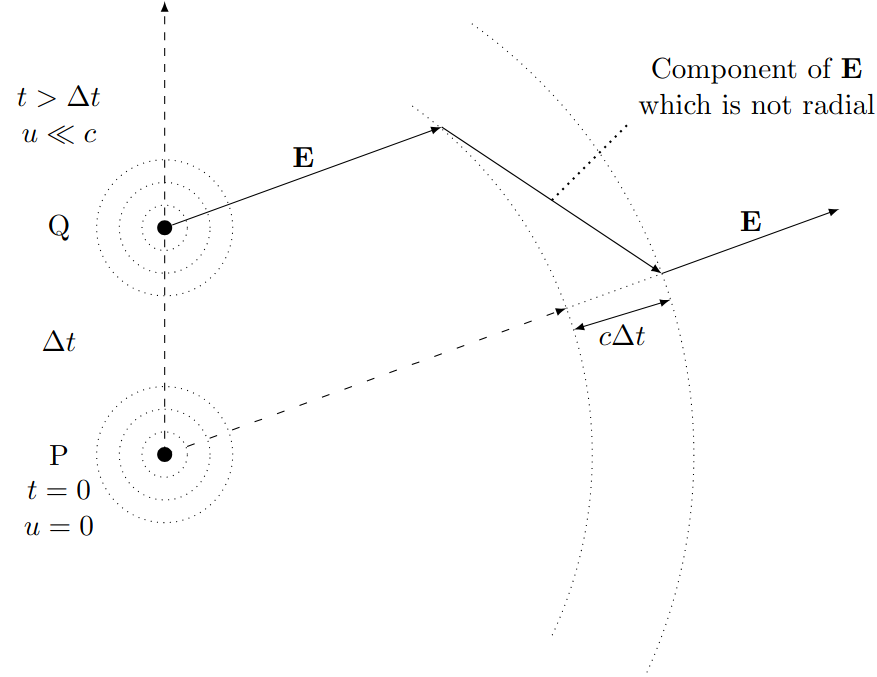
\includegraphics[width=0.75\textwidth]{2.3.png}
	\caption{}
	\label{fig:2.3}
\end{figure}
Consider figure \ref{fig:2.3}, initially at rest at point $P$ in free space. It is given a sudden impulse and undergoes a sudden acceleration $a$ over a short time $\Delta t$, such that when the charge reaches $Q$ it is moving at a constant velocity $u = a\Delta t << c$. If we consider the observer at a far away distance $r$, they will still see the charge at its original, stationary position. In order to see the charge move, the observer must wait a time $t = r/c$. In this time, there must be a boundary where the field configurations move from the old stationary state to the moving state. This boundary will have a width $c\Delta t$ and will must move away from the charge's location at a speed $c$.
\\\\
Let us recall that $\div{\vb{E}} = 0$, so there can be no discontinuities in the field lines generated by the charge. The boundary thus presents itself as a \textit{kink} in the electric field lines, as shown in figure \ref{fig:2.3}. This is a component of $\vb{E}$ which is not radial. 
\begin{figure}
	\centering
	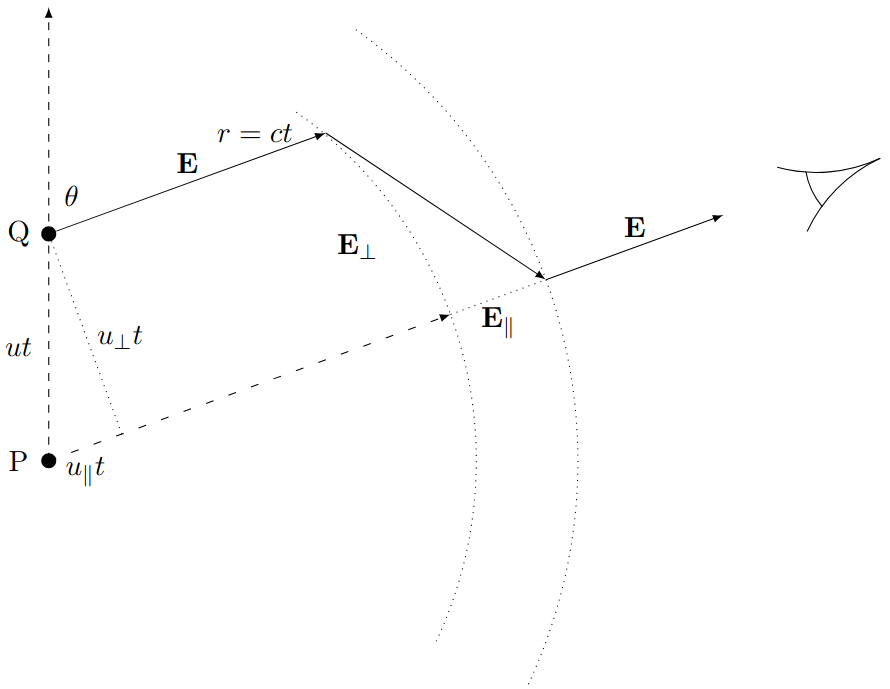
\includegraphics[width=0.75\textwidth]{2.4.png}
	\caption{}
	\label{fig:2.4}
\end{figure}
\\\\
Let us now consider the observer looking at the charge at some angle $\theta$ while it undergoes its final motion, reaching a position $ut$. Let us note that the boundary of observing the charge's motion is
\begin{equation}
	r = ct.
\end{equation}
According to the observer, the charge appears at $u_{\parallel}t$ parallel to their line of sight and  $u_{\perp}t$ perpendicular to their line of sight. We can then relate these to the parallel and perpendicular components of the kink $E_{\parallel}$ and $E_{\perp}$,
\begin{equation}
	\frac{E_{\perp}}{E_{\parallel}} = \frac{u_{\perp} t}{c\Delta t}.
\end{equation}  
If we note that $u_{\perp} = a_{\perp}\Delta t$, we can write,
\begin{equation}
	E_{\perp} = E_{\parallel}\frac{a_{\perp}r}{c^2}.
\end{equation}
Furthermore, since the charge's field is radial, we can say,
\begin{equation}
	E_{\parallel} = \frac{1}{4\pi\varepsilon_0}\frac{q}{r^2}
\end{equation}
so we can write,
\begin{equation}
	E_{\perp} = \frac{1}{4\pi\varepsilon_0}\frac{qa_{\perp}}{c^2r}.
\end{equation}
Let us summarise what we have found using this thought experiment,
\begin{enumerate}
	\item The field $E_{\perp} \propto 1/r$ in the kink region.
	\item Recalling equation \eqref{eq:A4}, we see $B_{\perp} = E_{\perp}/c$ in the kink region.
	\item The magnitude of the Poynting vector $\vb{S} = \frac{1}{\mu_0}\vb{E}\cross\vb{B}$ is, $S \propto EB \propto 1/r^2$
\end{enumerate}
which satisfy our conditions for radiation.
\subsection{Radiation pattern from a displaced point charge}
We wish to now consider the electric field and the power flux (Poynting vector) as time dependent functions, noting that we will require using the retarded time. By noting that $a_{\perp} = a \sin\theta$, we can simply write,
\begin{equation}
	\abs{\vb{E}(\vb{r},t)} = \frac{1}{4\pi\varepsilon_0}\frac{q\abs{\vb{a}\left(t - \frac{r}{c}\right)}\sin\theta}{c^2r}.
\end{equation}
Then, we can write the Poynting vector as,
\begin{equation}
	\abs{\vb{S}(\vb{r},t)} = \frac{1}{16\pi^2\varepsilon_0}\frac{q^2\abs{\vb{a}^2\left(t - \frac{r}{c}\right)}\sin^2\theta}{c^3r^2}. \label{eq:poynt}
\end{equation}
\subsection{Total Power Radiated}
The Poynting vector is the directional energy flux per unit area, per unit time. Thus, to find the power radiated, we simply compute the integral,
\begin{equation}
	P(t) = \oint \vb{S}\cdot\dd{\vb{A}} = \int_0^{2\pi}\int_0^{\pi} S r^2\sin\theta \dd{\theta} \dd{\phi}.
\end{equation}
Substituting expression \eqref{eq:poynt}, we obtain Larmor's formula,
\begin{equation}
	\boxed{P(t) = \frac{q^2\left[a\left(t-\frac{r}{c}\right)\right]^2}{6\pi \varepsilon_0c^3}}.
\end{equation}
\section{Radiation from an Oscillating Electric Dipole}
\begin{figure}
	\centering
	\begin{tikzpicture}
		\draw[<->] (0,0) -- (0,4);
		\node at (0,1) {\textbullet};
		\node at (0,3) {\textbullet};
		\node[anchor=west] at(0,1) {$q$};
		\node[anchor=west] at(0,3){$q$};
		\draw [->] (0,2) -- (2,2);
		\draw [latex-latex] (-0.5,1) -- (-0.5,3) node[midway, anchor=east] {$l$};
	\end{tikzpicture}
	\caption{}
	\label{fig:dipole}
\end{figure}
Consider an oscillating dipole, with charges separated by a length $l$ and oscillating along the $z$ axis. From Larmor's formula, $P(t) \propto \left(qa(\tau)\right)^2$. We can approximate the oscillating charges as a charge distribution with charge per unit length $\mu$ and length $l$. We can write,
\begin{equation}
	\begin{split}
		qa(\tau) & = \mu la(\tau) \\
		& = \mu \dv{v}{\tau}l \\
		& = l \dv{(\mu v(\tau))}{\tau}
	\end{split}
\end{equation}
where we find $\mu v(\tau)$ to have units of current, i.e., $\left[\mu v(\tau)\right] = [A]$. We can represent this as a current,
\begin{equation}
	\mu v (\tau) =  I(\tau) = I_0\cos\omega t
\end{equation}
where $I_0$ and $\omega$ are the corresponding amplitude and angular frequency of oscillation. Thus, we can write $qa(\tau)$ as,
\begin{equation}
	qa(\tau) = - \omega L I_0 \sin(\omega t - kr).
\end{equation}
By substitution, we can find the corresponding electric and magnetic fields,
\begin{align}
	E_{\perp} = \frac{I_0 l \sin\theta}{4\pi \varepsilon_0 rc^2}\omega \sin(\omega t - kr) && B_{\perp} = \frac{I_0 l \sin\theta}{4\pi \varepsilon_0 rc^3}\omega \sin(\omega t - kr) \label{eq:hertzian}
\end{align}
and the corresponding power emitted is,
\begin{equation}
	P = \left[\frac{l^2 \omega ^2}{6\pi \varepsilon c^3}\right]I_0 \sin^2(\omega t - kr). \label{eq:powerrad}
\end{equation}
\subsection{Radiation Resistance}
If we recall the formula $P = I^2 R$, we find that we can extract a resistance from equation \eqref{eq:powerrad}. This is known as the \textit{radiation resistance}, given by,
\begin{equation}
	R_{\text{rad}} = \frac{l^2 \omega ^2}{6\pi \varepsilon c^3}
\end{equation}
\section{Half-Wave Antenna}
\begin{figure}
	\centering
	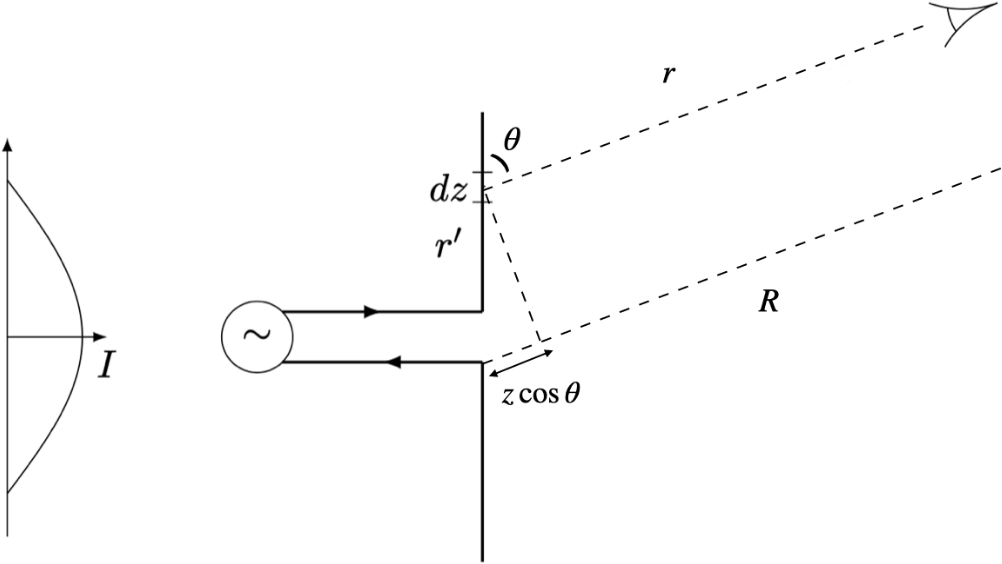
\includegraphics[width=0.5\textwidth]{2.6.png}
	\caption{}
	\label{fig:2.6}
\end{figure}
Let us consider a more realistic antenna, as in figure \ref{fig:2.6}. This is a centre fed, thin, straight antenna of length $l$. The solution for the current distribution of this antenna can be obtained from Maxwell's equations, whose solution is,
\begin{equation}
	I(z) = I_0 \sin\left(m\pi \left(\frac{\abs{z}}{l} + \frac{1}{2}\right)\right)
\end{equation}
where $m$ is an integer. We can integrate the Hertzian dipole over the length of the antenna in order to obtain an expression for the electric field, we have
\begin{equation}
	\dd E = \frac{I(z) \dd{z}\sin\theta}{4\pi \epsilon_0 r c^2}\omega \sin(\omega t - kr).
\end{equation}
Before we integrate this, we must consider the phase $\omega t - kr$. We find that there will be a time-lag of $\Delta t \frac{z\cos\theta}{c}$, with a resultant lag in phase of $kz\cos\theta$. Furthermore, we can approximate $r \approx R - z\cos\theta$, thus our integral becomes,
\begin{equation}
	E = \frac{\omega \sin\theta}{4\pi \varepsilon_0Rc^2}\int_{-l/2}^{l/2}I(z) \sin\left(\omega t - kR + kz\cos\theta\right)\dd{z}
\end{equation}
and computing this,
\begin{equation}
	E = \frac{I_0 l}{4\pi \varepsilon_0Rc^2}\left[\frac{2}{\pi}\frac{\cos\left(\frac{\pi}{2}\cos\theta\right)}{\sin\theta}\right]\omega \sin\left(\omega t - kR\right).
\end{equation}
We wish to then find the time-averaged poynting vector, computed by $\langle S \rangle = \frac{1}{\mu_0}\langle \vb{E}\cross\vb{B}\rangle$, which we find to be,
\begin{equation}
	\langle S \rangle = \frac{I_0^2}{8\pi^2 \mu_0\varepsilon_0^2R^2c^3}\frac{\cos^2\left(\frac{\pi}{2}\cos\theta\right)}{\sin^2\theta}.
\end{equation}
We can then compute the time average of the power radiated by $\langle P \rangle = \oint \langle S \rangle\dd{A}$, which requires us to compute,
\begin{equation}
	\langle P \rangle = \frac{I_0^2}{4\pi \mu_0\varepsilon_0^2 R^2c^3}\int_0^{\pi}\frac{\cos^2\left(\frac{\pi}{2}\cos\theta\right)}{\sin\theta}\dd{\theta}
\end{equation}
We then find,
\begin{equation}
	\langle P \rangle \simeq 1.22\frac{I_0^2}{r\pi \varepsilon_0 c} \simeq 0.194Z_0I_{\text{rms}}^2
\end{equation}
where we define $Z_0 = \frac{1}{\varepsilon_0 c} = \sqrt{\frac{\mu_0}{\varepsilon}}$ and $I_{\text{rms}} = \frac{I_0^2}{2}$.

\chapter{Radiation in Matter}
\section{Maxwell's Equations in a Medium}
Let us recall electromagnetic fields in materials. 
\subsection{Electrics}
The $\vb{P}$ field is the dipole moment per unit volume, and describes bound charges, such that,
\begin{align}
	\div{\vb{P}} = \rho_b && \vb{P}\cdot\vu{n} = \sigma_b
\end{align}
where $_b$ indicates a bound charge, and $\sigma_b$ is the bound surface charge. The total charge is composed of bound charge and free charge, such that $\rho = \rho_b + \rho_f$. We can then define the $\vb{D}$ field, such that,
\begin{equation}
	\div{\vb{D}} = \rho_f
\end{equation} 
for linear dielectrics, and,
\begin{equation}
	\vb{D} = \epsilon_0\vb{E} + \vb{P} = \epsilon_0\epsilon_r\vb{E}
\end{equation}
where $\epsilon_r = 1 + \chi_E$.
\subsection{Magnetics}
In magnetics, materials can have different types of magnetism:
\begin{itemize}
	\item \textit{Paramagnetism:} Magnetisation parallel to $\vb{B}$, dipoles align with $\vb{H}$.
	\item \textit{Diamagnetism:} Magnetisation is antiparallel with $\vb{B}$, dipoles anti-align with $\vb{H}$.
	\item \textit{Ferromagnetism:} Magnetisation is retained even after $\vb{B}$ is removed, regions of dipoles align together with $\vb{H}$.
\end{itemize}
We can define the magnetisation $\vb{M}$ as the magnetic dipole moment per unit volume, from which we can obtain the bound and surface currents,
\begin{align}
	\vb{j}_b = \curl{\vb{M}} && \vb{K}_b = \vb{M} \times \vu{n}.
\end{align}
We can then define a $\vb{H}$ field for free currents such that,
\begin{equation}
	\curl{\vb{H}} = \vb{J}_f
\end{equation}
where,
\begin{equation}
	\vb{H} = \frac{1}{\mu_0}\vb{B} - \vb{M} = \frac{1}{\chi_M}\vb{M} = \frac{1}{\mu_0\mu_r}\vb{B}.
\end{equation}
\subsection{Time dependent case}
\begin{align}
	\div{\vb{D}} = \rho_f && \div{\vb{B}} = 0\\
	\curl{\vb{H}} = \pdv{\vb{D}}{t} + \vb{j}_f && \curl{\vb{E}} = -\pdv{\vb{B}}{t}
\end{align}
\section{Plane Waves in Lossy Media}
Consider electromagnetic waves travelling in the $z$ direction such that,
\begin{align}
	\vb{E} = \left(E_x, 0, 0\right) && E_x = E_0e^{i(\omega t - kz)} \\
	\vb{B} = \left(0, B_y, 0\right) && B_y = B_0e^{i(\omega t - kz)}
\end{align}
Considering Faraday's law, we get,
\begin{equation}
	-ikE_0e^{i(\omega t - kz)} = -i\omega B_0 e^{i(\omega t - kz)}
\end{equation}
and thus,
\begin{equation}
	\frac{B_0}{E_0} = \frac{k}{\omega}.
\end{equation}
Recalling Ohm's law $\vb{J} = \sigma \vb{E}$ where $\sigma$ is the conductivity, and Ampere's law, we obtain,
\begin{equation}
	k^2 = \frac{\omega^2}{c^2} \epsilon_r\mu_r - i\omega \mu_r\mu_0 \sigma \label{eq:dispersion} 
\end{equation}
which is the dispersion relation for a linear, isotropic, dielectric medium. We see that this expression is complex, and reduces to the vacuum condition under vacuum. 
\subsection{Source-Free Lossy Media}
Let us consider a conducting media with dielectric properties and free current $\vb{J}_f$. Using Ampere's law,
\begin{equation}
	\begin{split}
		\curl{\vb{H}} & = \pdv{\vb{D}}{t} + \vb{J}_f \\
		& = i \omega \epsilon_0\epsilon_r \vb{E} + \sigma \vb{E} \\
		& = (i\omega \epsilon_0\epsilon_r + \sigma)\vb{E} \\
		& = i\omega(\epsilon_0\epsilon_r + \frac{\sigma}{i\omega})\vb{E}.
	\end{split}
\end{equation}
We can then define the \textit{complex permittivity},
\begin{equation}
	\epsilon_c = \epsilon_0\epsilon_r - \frac{i\sigma}{\omega}
\end{equation}
which we apply to conducting media. In the case of complex media, Ampere's law becomes $\curl{\vb{H}} = i\omega\epsilon_c\vb{E}$, but otherwise, we simply replace $\epsilon_0\epsilon_r$ with $\epsilon_c$ to retrieve Maxwell's equations for conducting media. We can then write down the source free Maxwell's equations,
\begin{align}
	\curl{\vb{E}} = -i\omega \mu \vb{H} && \curl{\vb{H}} = i\omega \epsilon\vb{E} \\
	\div{\vb{E}} = 0  && \div{\vb{H}} = 0.
\end{align}
By considering $\curl{\curl{\vb{E}}}$ we can derive the Helmholtz equation of electromagnetism.
\begin{equation}
	\laplacian{\vb{E}} + \omega^2\mu \epsilon \vb{E} = 0
\end{equation}
where we often parametrise $k_c^2 = \omega^2\mu\epsilon$.
\subsubsection{Transmission line theory}
We define the transmission line constant as,
\begin{equation}
	\gamma = ik_c = i\omega\sqrt{\mu\epsilon_c}
\end{equation}
which can be written in a general form,
\begin{equation}
	\gamma = \alpha + i \beta
\end{equation}
since its a complex number. We can then rewrite the Helmholtz equation as,
\begin{equation}
	\laplacian \vb{E} - \gamma^2 \vb{E} = 0
\end{equation}
from which we find that the electric field has a form,
\begin{equation}
	\vb{E} = E_0e^{i\omega t}e^{-\alpha z} e^{-i\beta z}
\end{equation}
where $e^{i\omega t}$ represents the oscillatory time dependence, $e^{-\alpha z}$ represents exponential attenuation, and $e^{-i\beta z}$ is a phase factor.
\section{Waves in Dielectrics}
In a dielectric $\mu_R \approx 1$ and $\sigma \approx 0$. Furthermore, the electrons will have bound electrons which will have spring-like forces holding them together in the dielectric. We can then model their motion as a forced-damped oscillator,
\begin{equation}
	\Ddot{\vb{x}} + \beta \Dot{\vb{x}} + \omega \vb{x} = \frac{q}{m}\vb{E}
\end{equation}
where $\beta$ is a damping constant. The solution to this equation is then,
\begin{equation}
	\vb{x} = \frac{\frac{q}{m}}{(\omega_0^2 - \omega^2)+i\beta\omega}\vb{E}
\end{equation}
where $\omega_0$ is the natural frequency of the electron. We know that the dipole moment of a single particle is given by $\vb{p} = q\vb{x}$, thus,
\begin{equation}
	\vb{p} = \frac{\frac{q^2}{m}}{(\omega_0^2 -\omega^2) + i \beta \omega}\vb{E}.
\end{equation}
The total magnetic moment will be given by a weighted sum of individual magnetic moments of each electron $\vb{P} = \sum_n^Nf_i\vb{p}_i$, so,
\begin{equation}
	\vb{P} = \sum_j \frac{Nf_j\left(\frac{q^2}{m}\right)}{(\omega_j^2 -\omega^2) +i\beta\omega} = \chi_E \epsilon_0 \vb{E}. 
\end{equation}
We can then write out the electric susceptibility, as well as rationalising the expression,
\begin{equation}
	\chi_E = \frac{q^2}{m\epsilon_0}\sum_j \frac{Nf_j(\omega_j^2 - \omega^2) - iNf_j\omega\beta}{(\omega_j^2 + \omega^2) + \omega^2 \beta^2}
\end{equation}
from which we see we are able to extract the real and imaginary part of the electric susceptibility, $\chi_E = \chi_R + i\chi_I$.
\subsection{Refractive Index of Gasses}
In a gas, we can write the refractive index as,
\begin{equation}
	n \simeq \sqrt{\epsilon_r}
\end{equation}
and given that $\epsilon_r = 1 + \chi_E$ and $n = \sqrt{1 + \chi_E} \approx 1 + \frac{\chi_E}{2}$ by binomial expansion, given $\chi_E$ is small, the refractive index is given by,
\begin{equation}
	n = 1 + \frac{\chi_{R}}{2} - i \frac{\chi_{I}}{2}
\end{equation}
from which we can define the real and imaginary refractive indexes,
\begin{align}
	n_R = 1 + \frac{\chi_{R}}{2} && n_I = \frac{\chi_{I}}{2}.
\end{align}
\begin{figure}
	\centering
	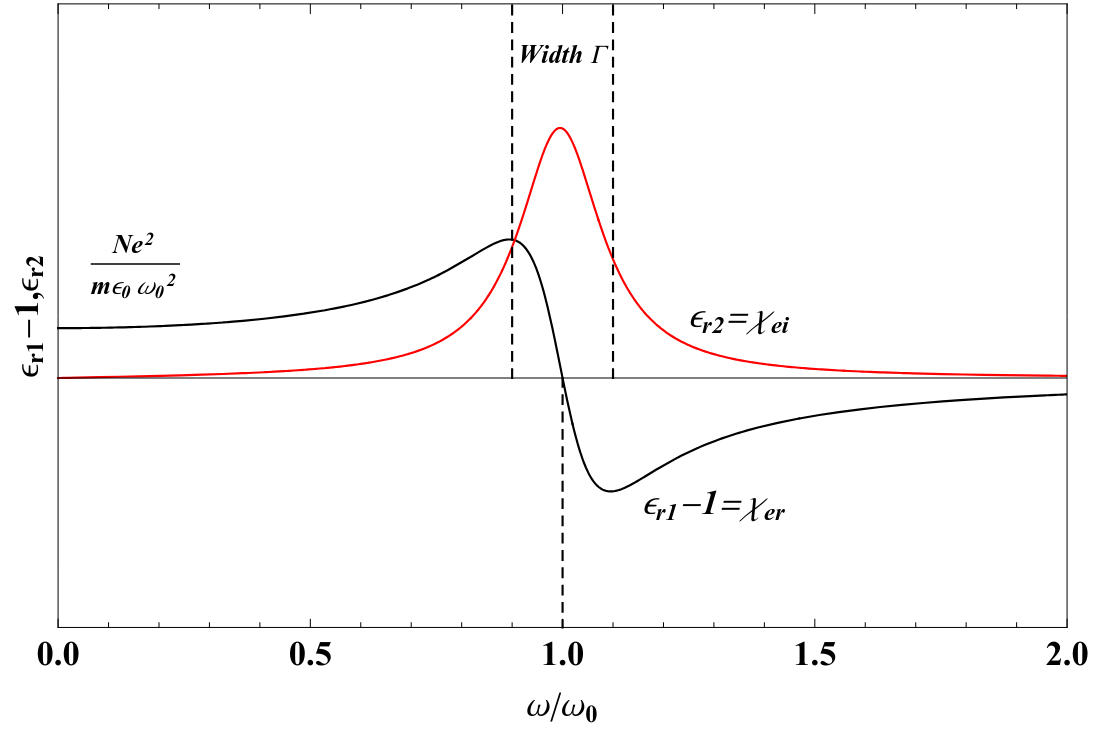
\includegraphics[width=0.5\textwidth]{realimg.png}
	\caption{The real and complex parts of permittivity for a a single resonant frequency $\omega_0$. In a dielectric there may be many such frequencies, which we label $\omega_j$.}
	\label{fig:gasses}
\end{figure}
In figure \ref{fig:gasses}, we visualise the real and imaginary parts of the refractive index for a given $\omega_0$. We describe observations below,
\begin{enumerate}
	\item $\omega = \omega_0$, refractive index is purely real, so we get maximum power transfer.
	\item $n_r > 1$, $\dv{n}{\omega} > 1$;
	\item $|\Gamma| < n_r$, $\dv{n}{\omega} < 1$;
	\item $n_r < 1$, $\dv{n}{\omega} > 0$;
	\begin{itemize}
		\item 1 and 3 are known as the \textit{normal dispersion regions} and 2 is known as the \textit{anomalous dispersion region}. 
	\end{itemize}
	
	\item In the limit $\omega \to 0$, we find,
	\begin{align}
		n_R \to 1 + \frac{q^2Nf_i}{2m\epsilon_0\omega_j^2} && n_I \to 0;
	\end{align}
	\item $n = c/v_p$, $v_p = \omega/k$, $n = ck/\omega$, and for some frequencies $n < 1$, in which case $\omega/k > c$
	\begin{itemize}
		\item However, $\dv{\omega}{k} < c$ always. 
	\end{itemize}
\end{enumerate}
\section{Waves in Conductors}
Metals and semiconductors have a lattice of fixed ions and electron gas, which are almost freely moving. Therefore, an external $\vb{E}$ field creates a current. We can the use Ohm's law $\vb{J} = \sigma \vb{E}$. We can rewrite the dispersion relation in equation \eqref{eq:dispersion} as,
\begin{equation}
	k_c = k_0\sqrt{\mu_r\epsilon_r}\sqrt{1 - i\frac{\sigma}{\epsilon_r \epsilon_0 \omega}} \label{eq:com}
\end{equation}
\subsection{Poor Conductors}
In poor conductors, we have that $\frac{\sigma}{\epsilon_r \epsilon_0\omega} <<1$, so we can perform a Taylor expansion on equation \eqref{eq:com},
\begin{equation}
	k_c \approx k_0 \sqrt{\mu_r\epsilon_r}(1 - \frac{i}{2}\frac{\sigma}{\epsilon_r \epsilon_0\omega}).
\end{equation}
Let us consider the modulus of the imaginary part of $k_c$,
\begin{equation}
	\abs{k_I} = \frac{\omega}{c}\sqrt{\mu_r\epsilon_r}\frac{\sigma}{2\epsilon_r \epsilon_0} = \frac{\sigma}{2}\sqrt{\frac{\mu_r\mu_0}{\epsilon_r\epsilon_0}}
\end{equation}
from which we can define the skin depth,
\begin{equation}
	\delta = \frac{1}{|k_I|} = 	\frac{2}{\sigma}\sqrt{\frac{\epsilon_r\epsilon_0}{\mu_r\mu_0}}.
\end{equation}
Let us recall the wavelength of light is given by,
\begin{equation}
	\lambda = \frac{2\pi}{\lambda} = \frac{2\pi c}{\omega}\frac{1}{\sqrt{\epsilon_r\mu_r}}.
\end{equation}
We are then interested in the ratio of the wavelength and skin depth, i.e., what fraction of the wavelength the wave can penetrate,
\begin{equation}
	\frac{\delta}{\lambda} = \frac{\omega}{\pi\sigma}\epsilon_r\epsilon_0
\end{equation}
and for a poor conductor, we find $\delta/\lambda << 1$. Therefore, an EM field can penetrate many wavelengths through a poor conductor before it decays.
\subsection{Good Conductors}
We now expect, $\frac{\sigma}{\omega\epsilon_o\epsilon_r} >> 1$. The dispersion relation \eqref{eq:dispersion} now reduces to,
\begin{equation}
	\begin{split}
	k_c & = \sqrt{\mu_r\epsilon_r}\sqrt{\frac{\omega\sigma}{\epsilon_r\epsilon_0}}\sqrt{\epsilon_0\mu_0}\underbrace{(-i)^{1/2}}_{\frac{1}{\sqrt{2}}(1-i)} \\
	& = \sqrt{\frac{\mu_r\mu_0\sigma\omega}{2}}(1-i)
\end{split}
\end{equation}
and thus,
\begin{align}
	\delta = \sqrt{\frac{2}{\mu_r\mu_0\sigma\omega}} &&\lambda = \frac{2\pi}{k_R} = 2\pi\delta
\end{align}
so,
\begin{equation}
	\frac{\sigma}{\lambda} = \frac{1}{2\pi} \sim 0.16
\end{equation}
so most of the wave is absorbed by a good conductor. Furthermore, if we calculate,
\begin{equation}
	\frac{B}{E} \sim \frac{k}{\omega} = \sqrt{\frac{\mu_r\mu_0\sigma}{\omega}}\underbrace{\frac{1}{\sqrt{2}}(1-i)}_{e^{-i\frac{\pi}{4}}}
\end{equation}
so the magnetic and electric field have a phase difference of $45^{\text{o}}$ in a conductor.
\section{Waves in Plasmas}
In a plasma, we have free electrons moving in the presence of stationary positive and neutral ions. We will consider the motion of the electrons in a plasma.
\subsection{The Drude Model}
We will consider the collisions in the plasma to be elastic. Since the electrons are also unbound, our equation of motion becomes,
\begin{equation}
	-e\vb{E} = m\dv[2]{\vb{x}}{t} = -k\vb{x}.
\end{equation}
We have that $\omega = \sqrt{k/m} \implies k = \omega^2m$, so,
\begin{equation}
	-e\vb{E} = -\omega^2m\vb{x} \implies \vb{x} = \frac{e}{m\omega^2}\vb{E}
\end{equation}
which is the electron displacement. Such a displacement causes a dipole moment,
\begin{equation}
	\vb{p} = - e\vb{x}
\end{equation}
and polarisation,
\begin{equation}
	\vb{P} = n\vb{p} = -\frac{Ne^2}{m\omega^2}\vb{E}
\end{equation}
from which we ca obtain our $\vb{D}$ field,
\begin{equation}
	\vb{D} = \epsilon_0\vb{E} + \vb{P} = \epsilon_0\left(1 - \frac{Ne^2}{m\omega^2\epsilon_0}\right)\vb{E}
\end{equation}
and thus we have found an equivalent $\epsilon_r$ for plasma. We can further define a \textit{plasma frequency},
\begin{equation}
	\omega_p^2 = \frac{Ne^2}{m\epsilon_0}
\end{equation}
so that,
\begin{equation}
	\vb{D} = \epsilon_0\left(1-\frac{\omega_p^2}{\omega^2}\right)\vb{E}.
\end{equation}
Collisions give rise to an average velocity of electrons, and this mechanism will cause a damping term in the equation of motion. If we consider $\gamma_c$ to be the collision frequency and $\tau_c = 1/\gamma_c$ to be the collision time, we can obtain a current by,
\begin{equation}
	\vb{J} = \omega_0 \vb{E} = -Ne\vb{v}_{\text{drift}}
\end{equation}
where we can define,
\begin{align}
	\vb{v}_{\text{drift}} = -\frac{e\vb{E}}{m}\frac{1}{\gamma_c} && \sigma_0 = \frac{Ne^2}{m}\frac{1}{\gamma_c} = \frac{\epsilon_0\omega_p^2}{\gamma_c}.
\end{align}
\subsection{Drude Model with Collisions}
Let us now consider inelastic collisions in a plasma. We add a damping term $\beta$ to our equation of motion,
\begin{equation}
	m\Ddot{\vb{x}} + m\beta\Dot{\vb{x}} = -e\vb{E}_0e^{i\omega t}
\end{equation}
from which we obtain a displacement,
\begin{equation}
	\vb{x} = \frac{-\frac{e}{m}}{-\omega^2 + i\omega\beta}\vb{E}_0e^{i\omega t}
\end{equation}
and velocity,
\begin{equation}
	\Dot{x} = \frac{-ie\frac{\omega}{m}}{-\omega^2 + i\omega\beta}\vb{E}_0e^{i\omega t}
\end{equation}
We will then have a current,
\begin{equation}
	\vb{J} = \sigma(\omega)\vb{E} = -Ne\Dot{x}
\end{equation}
such that,
\begin{equation}
	\sigma(\omega) = \frac{\sigma_0}{1 + i\frac{\omega}{\gamma_c}}
\end{equation}
where we define the DC conductivity,
\begin{equation}
	\sigma_0 = \frac{Ne^2}{m}\frac{1}{\gamma_c}.
\end{equation}
Let us investigate the permittivity. Using $\vb{P}  = N(-e)\vb{x}$ from the Drude model, we find,
\begin{equation}
	\chi_E = \frac{Ne^2}{\epsilon_0m}\frac{1}{-\omega^2 + i\gamma_c\omega}
\end{equation}
and $\epsilon_r = 1 + \chi_E$ so,
\begin{equation}
	\epsilon_r = 1+ \frac{\omega_p^2}{-\omega^2 + i\gamma_c\omega}. \label{eq:perm}
\end{equation}
\subsubsection{Low frequency waves in plasma}
If we consider $\omega << \gamma_c$, we reduce equation \eqref{eq:perm} to,
\begin{equation}
	\epsilon_r = 1+ \frac{\sigma_0}{i\omega\epsilon_0} \simeq -i\frac{\sigma_0}{\omega\epsilon_0}.
\end{equation}
The refractive index is then,
\begin{equation}
	n = \sqrt{\epsilon_r} = \sqrt{\frac{\sigma_0}{\omega\epsilon_0}}\sqrt{-i} = \sqrt{\frac{\sigma_0}{2\omega\epsilon_0}}(1-i)
\end{equation}
so we find $n_R = n_I$. We then find the skin depth to be,
\begin{equation}
	\sigma = \sqrt{\frac{2}{\mu_0\sigma_0\omega}}.
\end{equation}
\subsubsection{High frequency waves in plasma}
For a high frequency wave, $\omega >> \gamma_c$, we find,
\begin{equation}
	\epsilon_r \simeq 1 - \frac{\omega_p^2}{\omega^2}.
\end{equation}
We can then extract the dispersion relation for a plasma,
\begin{align}
	\omega^2 = k^2c^2 + \omega_p^2\\
	k = \pm\frac{1}{c}\left(\omega^2 + \omega_p^2\right)^{\frac{1}{2}}
\end{align}
we then find that $\epsilon_r$ is real no matter the value of $\omega$, EM waves travel through plasmas as if through vacuum. Let us consider some limiting situations with frequency,
\begin{enumerate}
	\item $\omega = \omega_p \implies k = 0$, and we find, $k \to 0 \implies v_p \to \infty$ and $v_g \to 0$, so the wave ceases to propagate.
	\item $\omega >> \omega_p$
	\item $\omega << \omega_p$, we find that $k$ is purely imaginary and described by,
	\begin{equation}
		kc = -i\sqrt{\omega_p^2 -\omega^2}
	\end{equation}
	and the electromagnetic wave undergoes an exponential decay.
\end{enumerate}
\chapter{Reflection and Refraction}
\section{Maxwell's Equations and Boundary Conditions}
We will consider the boundary conditions for $\vb{H}, \vb{B}, \vb{E},$ and $\vb{D}$  by Maxwell's equations.
\subsection{Transverse Component of Electric Field}
\begin{figure}[h]
	\centering
	\begin{tikzpicture}[scale=1.5]
		\draw (0,0) -- (5,0);
		\fill[pattern={Lines[angle = 45, distance=0.1cm]}] (0,0) rectangle (5, -0.1);
		\draw[-latex] (1,2) -- (2.5,0) node[anchor=south west] {$\vb{E}_1$};
		\draw[-latex, dashed] (1, 2) -- (1,0) node[anchor=south west] {$\vb{E}_{1\parallel}$};
		\draw[-latex, dashed] (1,2) -- (2.5,2) node[anchor=west] {$\vb{E}_{1\perp}$};
		\draw[-latex, color=blue] (2.5,0) -- (3, -1.5) node[anchor = north west] {$\vb{E}_2$};
		\draw[-latex, color=blue, dashed] (2.75,-0.75) -- (2.75, -1.5) node[anchor = north] {$\vb{E}_{2\parallel}$};
		\draw[-latex, color=blue, dashed] (2.75,-0.75) -- (3,-0.75) node[anchor = west] {$\vb{E}_{2\perp}$};
		\begin{scope}[thick, dashed, color = red, decoration={
				markings,
				mark=at position 0.5 with {\arrow{>}}}
			] 
		\draw[postaction={decorate}] (0.75,-1) -- (4.25,-1);
		\draw[postaction={decorate}]  (4.25,-1) -- (4.25,1) node[anchor=south west] {$C$};
		\draw[postaction={decorate}]	 (4.25,1) -- (0.75, 1);
		\draw[postaction={decorate}]	 (0.75, 1)-- (0.75, -1);
		\end{scope}
		\node[anchor=south west] at (0,0) {$\epsilon_1,\mu_1$};
		\node[anchor=north west] at (0,-0.1) {$\epsilon_2,\mu_2$};
		\draw[thick, decoration={brace,mirror,raise=5pt},decorate] (4.25,-1) -- (4.25,1) node[midway, right=6pt, anchor = south west] {$\Delta H$};
		\draw[thick, decoration={brace,mirror,raise=5pt},decorate] (4.25,1)--(0.75,1) node[midway, above=6pt] {$\Delta W$};
	\end{tikzpicture}
	\caption{}
	\label{fig:trans E}
\end{figure}\noindent
Let us consider a setup as in figure \ref{fig:trans E}, where an electric field is travelling through a material with $\epsilon = \epsilon_1$ and $\mu = \mu_1$ incident on the surface of a material with $\epsilon = \epsilon_2$ and $\mu = \mu_2$. Let us consider Ampere's law over a loop $C$ with width $\Delta W$ and height $\Delta H$,
\begin{equation}
	\oint_C \vb{E}\cdot\dd\vb{l} = -\pdv{t}\oint\vb{B}\cdot\dd\vb{S}
\end{equation}
which we can evaluate,
\begin{equation}
	\begin{split}
	& E_{2\perp}\Delta W - E_{1\perp}\Delta W + E_{1\parallel}\frac{\Delta H}{2} -  E_{1\parallel}\frac{\Delta H}{2} +  E_{2\parallel}\frac{\Delta H}{2} - E_{2\parallel}\frac{\Delta H}{2} = -\pdv{B}{t}\Delta H \\
	\implies & E_{2\perp} - E_{1\perp} = -\pdv{B}{t}\Delta H.
	\end{split}
\end{equation}
At the boundary, we take $\Delta H \to 0$, so,
\begin{align}
	E_{2\perp} &= E_{1\perp} \label{eq:Eperp} \\
	\frac{D_{2\perp}}{\epsilon_2} &= \frac{D_{1\perp}}{\epsilon_1}.
\end{align}

\begin{figure}[h]
	\centering
	\begin{tikzpicture}[scale=1.25]
		\begin{scope}[canvas is xy plane at z=1.5]
			\draw (0,0)arc (-30:30:-5);
		\end{scope}
		\begin{scope}[canvas is xy plane at z = -1.5]
			\draw (0,0) arc (-30:30:-5);
		\end{scope}
		\draw (0,0,1.5) -- (0,0,-1.5);
		\draw (0,-5,1.5) -- (0,-5,-1.5); 
		\begin{scope}[canvas is xy plane at z = 0]
			\draw[latex-] (-0.66987,-2.5) -- (-3,-1) node[anchor=south east] {$\vb{D}_1$};
			\draw[dotted] (-4,-2.5) -- (3.33013,-2.5);
			\draw[-latex, color=blue] (-0.66987,-2.5) -- (2.33,-3.5) node[anchor=north west] {$\vb{D}_2$};
			\draw[dashed, red] (-2,-3.5) -- (1.83013, -3.5);
			\draw[dashed, red] (-2,-1.5) -- (1.83013, -1.5);
			\draw[thick, decoration={brace,mirror,raise=5pt},decorate] (-2,-3.5) -- (1.83013, -3.5) node[midway, below=6pt] {$\Delta W$};
			\draw[thick, -stealth] (-2,-2.5) -- (-3.5,-2.5) node[anchor=south east] {$\vb{a}_{1\perp}$};
			\draw[thick, -stealth] (1.83013, -2.5) -- (3.33013, -2.5) node[anchor=west] {$\vb{a}_{2\perp}$};
			\draw[dashed, thick, blue, -latex] (-0.66987, -2.5) -- (0.8, -2.5) node[anchor=south] {$\vb{D_{2\parallel}}$};
			\draw[dashed, thick, blue, -latex] (-0.66987, -2.5) -- (-0.66987, -3) node[anchor=west] {$\vb{D_{2\perp}}$};
			\draw[dashed, thick, -latex] (-3,-1) -- (-2, -1) node[anchor=west] {$\vb{D_{1\parallel}}$};
			\draw[dashed, thick, -latex] (-3,-1) -- (-3, -1.5) node[anchor=east] {$\vb{D_{1\perp}}$};
		\end{scope}
		\begin{scope}[canvas is yz plane at x=-2]
			\filldraw[dashed, red, pattern={Hatch[angle=45, distance=0.2cm]}, pattern color=red] (-2.5,0) circle (1cm);
		\end{scope}
		\begin{scope}[canvas is yz plane at x=1.83013]
			\filldraw[dashed, red, pattern={Hatch[angle=45, distance=0.2cm]}, pattern color=red] (-2.5,0) circle (1cm);
		\end{scope}
		\node at (2.5,-2,0) {$\Delta S$};
		\node at (-1, 0, 0) {$\epsilon_1,\mu_1$};
		\node at (1, 0, 0) {$\epsilon_2,\mu_2$};
	\end{tikzpicture}
	\caption{}
	\label{fig:normal}
\end{figure}\noindent
\subsection{Normal (to interfacing surface) component of $\vb{D}$}
Let us consider a setup as in figure \ref{fig:normal}, where we have a $\vb{D}$ travelling through a material with $\epsilon = \epsilon_1$ and $\mu = \mu_1$ incident on the surface of a material with $\epsilon = \epsilon_2$ and $\mu = \mu_2$. We will consider Gauss' law, considering a cylinder of length $\Delta W$ and end surfaces of area $\Delta S$, 
\begin{equation}
	\oint_S\vb{D}\cdot\dd{\vb{S}} = Q.
\end{equation}
As we take $\Delta W \to 0$, the volume charge approaches a surface charge. We have that $\vb{a}_{1\perp} = -\vb{a}_{2\perp}$, so, for a surface charge density $\rho_S$,
\begin{equation}
	\begin{split}
		& \vb{a}_{2\perp}\cdot(\vb{D}_1 - \vb{D}_2)\Delta S = \rho_S\Delta S \\
		\implies & D_{1\parallel} - D_{2\parallel} = \rho_S
	\end{split}
\end{equation}
so the normal component of the electric field is discontinuous across the boundary.
\subsection{Transverse component of $\vb{H}$}
We will consider a similar setup to what we did for the transverse component of $\vb{E}$, but we will now consider the following equation,
\begin{equation}
	\begin{split}
		&\oint_C \vb{H}\cdot\dd{\vb{l}} = \oint \vb{J}\cdot \dd{S} + \pdv{t}\oint_S\vb{D}\cdot\dd{\vb{S}}\\
		\implies & H_{2\perp} -H_{2\perp} = J\Delta H + \pdv{D}{t}\Delta H
	\end{split}
\end{equation}
where, in the limit $\Delta H \to 0$, $J\Delta H \to J_z$ which is the sheet current, and $\pdv{D}{t}\Delta H \to 0$. We thus have,
\begin{equation}
	H_{2\perp} - H_{2\perp} = J_z. \label{eq:bperp}
\end{equation} 
\subsection{Normal of $\vb{B}$}
We can consider a similar setup to $\vb{D}$, considering Gauss' law for magnetic fields,
\begin{equation}
	\begin{split}
	&\oint\vb{B}\cdot\dd{\vb{S}} = 0 \\
	\implies & \vb{a}_{2\perp}\cdot(\vb{B}_1 - \vb{B}_2)\Delta S = 0 \\
	\implies & B_{1\parallel} = B_{2\parallel} \implies \vu{n}\cdot\vb{B} = 0
	\end{split}
\end{equation}
so the normal of $\vb{B}$ is continuous across the boundary.
\section{Reflection at Normal Incidence at a Plane Dielectric Boundary}
If we consider a a plane wave travelling from one medium $(\epsilon_1, \mu_1)$ into another medium $(\epsilon_2, \mu_2)$, we can write down the magnetic and electric components which are incident, reflected, and transmitted at the boundary,
\begin{align}
	E_i = E_{i_0}e^{i(\omega t - kz)} && B_i = B_{i_0}e^{i(\omega t - kz)} \\
	E_r = -E_{r_0}e^{i(\omega t + kz)} && B_r = B_{r_0}e^{i(\omega t + kz)}\\
	E_t = E_{t_0}e^{i(\omega t - kz)} && B_t = B_{t_0}e^{i(\omega t - kz)}
\end{align}
We wish to find the ratios between the incoming wave and the reflected and transmitted waves. Let us consider the mediums to be intercepting along the $x$-axis, and that the boundary is charge and current free. By equations \eqref{eq:Eperp} and \eqref{eq:bperp}, we obtain,
\begin{align}
	E_{i_0} - E_{r_0} & = E_{t_0} \label{eq:ET} \\
	\frac{B_{i_0}}{\mu_1} + \frac{B_{r_0}}{\mu_1} & = \frac{B_{t_0}}{\mu_2}.
\end{align}
We have that, $B = E/v = E\sqrt{\epsilon_0\epsilon_r\mu_0\mu_r} \implies B/\mu_r = E\sqrt{\epsilon_0\epsilon_r\mu_0\mu_r}\frac{1}{\mu_r} = \frac{1}{c}\sqrt{\frac{\epsilon_r}{\mu_r}}E$, $\mu_1 = \mu_2 = 0$ in a dielectric, and $\sqrt{\epsilon_1} = n_1$ and $\sqrt{\epsilon_2} = n_2$, so
\begin{equation}
	\begin{split}
		& \sqrt{\epsilon_1}E_{i_0} + \sqrt{\epsilon_1}E_{r_0} = \sqrt{\epsilon_2}E_{t_0} \\
		\implies & n_1(E_{i_0} + E_{r_0}) = n_2E_{t_0} \\
		\implies & \boxed{\frac{E_{r_0}}{E_{i_0}} = \frac{n_2 - n_1}{n_1 + n_2}}
	\end{split}
\end{equation} 
which is the reflection ratio. By using equation \eqref{eq:ET} to write $E_{r_0}$ in terms of $E_{t_0}$, we find,
\begin{equation}
	\boxed{\frac{E_{t_0}}{E_{i_0}} = \frac{2n_1}{n_1 + n_2}}
\end{equation}
which is known as the transmission ratio. These ratios hold for $B$ in the exact same way.
\subsection{Transmission and Reflection Coefficients}
To be able to consider the transmission and reflection coefficients, we have to consider the incident, reflected, and transmitted Poynting vector. We must first consider the average incident Poynting vector. This is given by,
\begin{equation}
	\langle S_i \rangle = \frac{1}{\mu_0}\langle \vb{E} \cross \vb{B}\rangle = \frac{1}{\mu_0}E_iB_i
\end{equation}
this then implies that $\langle S \rangle S \propto En^2$ generally. We can then say that,
\begin{align}
	\langle S_r\rangle \propto \left(\frac{n_2 - n_1}{n_1 + n_2}\right)^2n_1 \\
	\langle S_t \rangle \propto \left(\frac{2n_1}{n_1 + n_2}\right)^2n_2 \\
	\langle S_i \rangle \propto n_1 
\end{align}
thus,
\begin{align}
	\boxed{\mathcal{T} = \frac{4n_1n_2}{(n_1+n_2)^2}} \\
	\boxed{\mathcal{R} = \left(\frac{n_2 - n_1}{n_1 + n_2}\right)^2 }
\end{align}
which are the transmission and reflection coefficients, respectively.
\section{Reflection and Normal Incidence From a Conductor}
For a good conductor, we have that $\sigma >> 1$. We can write the refractive index in the conductor medium is,
\begin{equation}
	n_2 = \sqrt{\epsilon_r} = \sqrt{-i\frac{\sigma}{\omega\epsilon_0}} = \sqrt{\frac{\sigma}{2\omega\epsilon_0}}(1 - i)
\end{equation}
\section{Oblique Incidence}
\begin{figure}[h]
	\centering
	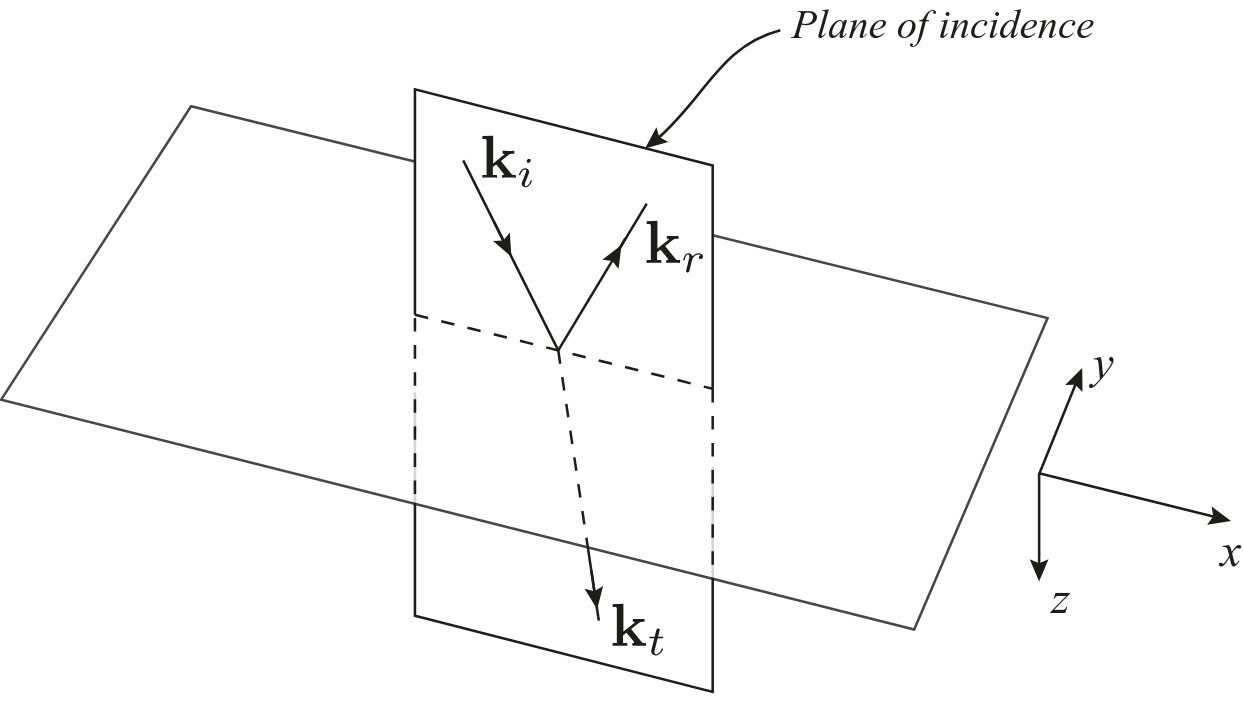
\includegraphics[width=0.6\textwidth]{oblique incidence.png}
	\caption{The wavevectors $\vb{k}_i$, $\vb{k_r}$ and $\vb{k}_t$ all lie in the same plane, i.e., the plane of incidence.}
	\label{fig:oblique}
\end{figure}
\subsection{Snell's Law}
Consider a wave incident on a surface as in figure \ref{fig:oblique}. Let us consider the electric field,
\begin{align}
	E_i = E_{i_0}e^{i(\omega t - \vb{k}_i\cdot{\vb{r}})} && E_r = E_{r_0}e^{i(\omega t - \vb{k}_r\cdot{\vb{r}})} && E_t = E_{t_0}e^{i(\omega t - \vb{k}_t\cdot{\vb{r}})} 
\end{align}
At the boundary, $z = 0$, the waves all have the same phase,
\begin{align}
	\eval{\vb{k}_i\cdot\vb{r}}_{z=0} = \eval{\vb{k}_r\cdot\vb{r}}_{z=0} = \eval{\vb{k}_t\cdot\vb{r}}_{z=0}
\end{align}
and thus, at $z = 0$,
\begin{equation}
	K_{i_x} x = k_{r_x}x = k_{t_x}x.
\end{equation}
Furthermore,
\begin{align}
	k_{i_x} = k_i \sin\theta_i,\label{eq:kti} \\
	k_{r_x} = k_r \sin\theta_r, \\
	k_{t_x} = k_t \sin\theta_t. \label{eq:ktx}
\end{align}
Due to the nature of reflection, $\theta_i = \theta_r$. Recall that $k = n\frac{\omega}{c}$, so,
\begin{equation}
	\boxed{n_1\sin\theta_i = n_2\sin\theta_t}
\end{equation}
and we have obtained Snell's law.
\subsection{Oblique Incidence of Polarised Light}
\begin{figure}[h]
	\centering
	\begin{subfigure}{0.4\textwidth}
		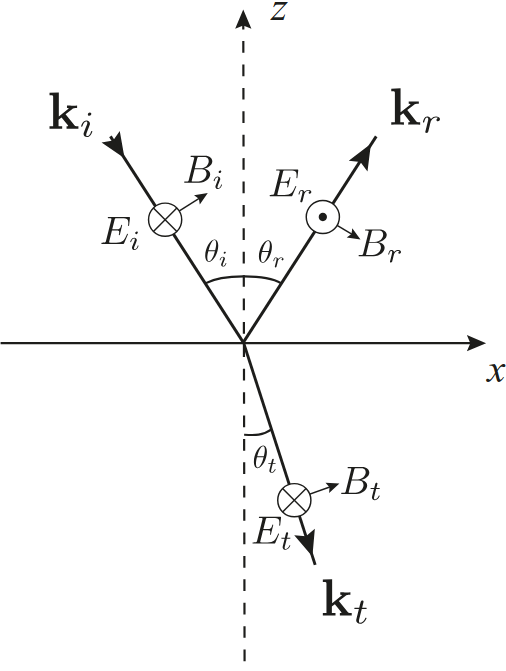
\includegraphics[width=0.9\linewidth]{S-polar.png}
		\caption{S-polarised oblique incidence (wave perpendicular to plane of incidence).}
	\end{subfigure}
	\begin{subfigure}{0.4\textwidth}
		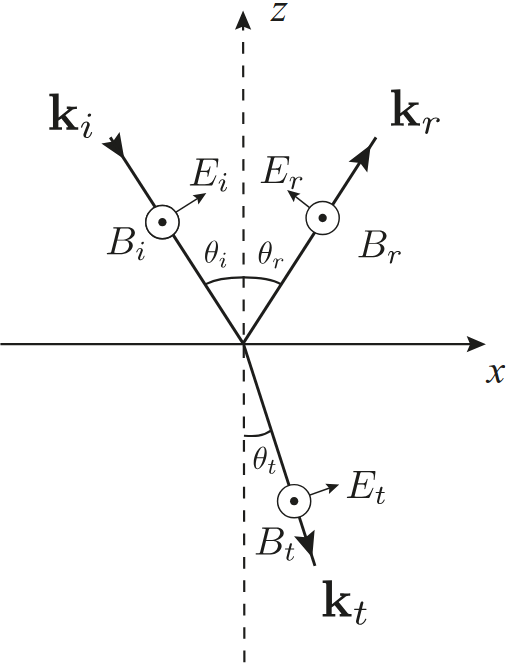
\includegraphics[width=0.9\linewidth]{p-polar.png}
		\caption{P-polarised oblique incidence (wave parallel to plane of incidence).}
	\end{subfigure}
	\caption{The directions of the electric and magnetic field components for $S$-polarised and $P$-polarised
		light.}
\end{figure}
Let us now consider light with different polarisations. We will consider $S$-polarised light (the $S$ stands for the German word for perpendicular) and $P$-polarised light ($P$ stands for parallel). 
\subsubsection{S-polarised light}
Considering $S$-polarised light first, we have that $E_t$ and $H_t$ are continuous, provided there is no current and we are not considering a perfect conductor. We then have that,
\begin{align}
	E_{i_0} - E_{r_0} &= E_{t_0}, \label{eq:b2}\\
	H_i\cos\theta_i + H_i\cos\theta_r &= H_t\cos\theta_t. \label{eq:b1}
\end{align}
Recall that $H = n\frac{E}{c}$, so, from boundary condition \eqref{eq:b1},
\begin{equation}
	n_1E_{i_0}\cos\theta_i + n_2E_{r_0}\underbrace{\cos\theta_r}_{\cos\theta_i} = n_2\underbrace{E_{t_0}}_{\eqref{eq:b2}} \cos\theta_t,
\end{equation}
and rearranging,
\begin{equation}
	\frac{E_{r_0}}{E_{i_0}} = -\frac{n_1\cos\theta_i - n_2 \cos\theta_t}{n_1\cos\theta_i + n_2\cos\theta_t}.
\end{equation}
By Snell's law, defining $n = n_2/n_1$, we can write down the \textit{reflection coefficient of an $S$-polarised wave},
\begin{equation}
	\rho_{\perp} \equiv \abs{\frac{E_{r_0}}{E_{i_0}}} = \abs{\frac{\cos\theta_i - \sqrt{n^2 - \sin^2\theta_i}}{\cos\theta_i + \sqrt{n^2 + \sin^2\theta_i}}}
\end{equation}
and the corresponding transmission coefficient is given by,
\begin{equation}
	\tau_{\perp} = \abs{\frac{E_{t_0}}{E_{i_0}}} = 1 - \rho_{\perp}.
\end{equation}
\subsubsection{P-polarised light}
We still have $E_t$ and $H_t$ being continuous, and we have,
\begin{align}
	E_i\cos\theta_i - E_{r_0}\cos\theta_i &= E_t\cos\theta_t, \\
	B_{i_0} + B_{r_0} &= B_{t_0}.
\end{align}
Recall $B = n \frac{E}{c}$, 
\begin{align}
	&n_1 E_{i_0} + n_1 E_{r_0} = n_2E_{t_0} \\
	&E_{t_0} = \frac{n_1}{n_2}(E_{i_0} + E_{r_0}).
\end{align}
We can then write,
\begin{equation}
	E_{i_0} \cos\theta_i - E_{r_0}\cos\theta_r = \frac{n_2}{n_1}(E_{i_0} + E_{r_0})\cos\theta_t
\end{equation}
and rearranging,
\begin{equation}
	\frac{E_{r_0}}{E_{i_0}} = \frac{n_2\cos\theta_i - n_1\cos\theta_t}{n_2\cos\theta_i + n_1\cos\theta_t}.
\end{equation}
Now using the same tick as before, we find the \textit{reflection coefficient of a $P$-polarised wave},
\begin{equation}
	\rho_{\parallel} = \abs{\frac{E_{r_0}}{E_{i_0}}} = \abs{\frac{n^2\cos\theta_i - \sqrt{n^2 - \sin^2\theta_i}}{n^2\cos\theta_i + \sqrt{n^2 - \sin^2\theta_i}}}
\end{equation}
and the corresponding transmission coefficient is given by,
\begin{equation}
	\tau_{\parallel} = \abs{\frac{E_{t_0}}{E_{i_0}}} = 1 - \rho_{\parallel}
\end{equation}
\subsection{Fresnel's Equations}
We define the impedance of free space as,
\begin{equation}
	Z_0 = \sqrt{\frac{\mu_0}{\varepsilon_0}} = \frac{E}{H}.
\end{equation}
We can define the impedance of a material by,
\begin{equation}
	Z = \frac{Z_0}{n}.
\end{equation}
We can then write the reflection coefficients of $S$ and $P$ polarised light in terms of impedance of the materials to obtain \textit{Fresnel's equations}.
\begin{tcolorbox}[title=Fresnel Equations]
	\begin{align}
	\rho_{\perp} & = \frac{Z_2\cos\theta_i - Z_1 \cos\theta_1}{Z_2 \cos\theta_i + Z_1 + \cos\theta_t} \\
	\rho_{\parallel} & = \frac{Z_1\cos\theta_i - Z_2 \cos\theta_t}{Z_1\cos\theta_i + Z_2\cos\theta_t}
	\end{align}
\end{tcolorbox}
\subsection{Brewster Angle}
For $P$-polarised light, we have that,
\begin{equation}
	\begin{split}
		n^2 \cos\theta_i &= \sqrt{n^2 - \sin^2\theta_i} \\
		n^4 \cos\theta_i & = n^2 - \sin^2\theta_i \\
		& = n^2 - 1 + \cos^2\theta_i \\
		(n^4 -1)\cos^2\theta_i & = n^2 -1 \\
		\cos\theta_i & = \frac{1}{\sqrt{1 +n^2}} \implies n^2= \frac{\sin^2\theta_i}{\cos^2\theta_i} \implies n = \tan\theta_i 
	\end{split}
\end{equation}
so, we can define the Brewster angle,
\begin{equation}
	\boxed{\theta_b = \arctan(n)}
\end{equation}
which is the angle where only the perpendicular component of randomly polarised light is reflected from a surface.
\subsection{Total Internal Reflection}
Total internal reflection occurs when light travels from a dense material to a rare material ($n_1 > n_2$), and is incident at an angle $\theta_c$ such that the transmitted angle is $90^{\text{o}}$. So, by Snell's law, the critical angle is,
\begin{equation}
	\boxed{\theta_c = \arcsin\left(n\right)}.
\end{equation}
For angles greater than the critical angle, we find that the Fresnel equations become complex. The perpendicular coefficient is given by
\begin{equation}
	\rho_{\perp} = \frac{A + iB}{A - iB}
\end{equation}
and we fin that the reflected intensity ratio is,
\begin{equation}
	R_{\perp} = \abs{\frac{A+iB}{A-iB}}^2 = 1
\end{equation}
i.e., the wave is totally reflected. However{, even though the wave is totally reflected, some of the wave is still transmitted. We can write the transmitted angle as,
\begin{equation}
	\cos\theta_t = \pm i \sqrt{\left(\frac{\sin\theta_t}{\sin\theta_i}\right)^2 - 1} = \pm i Q.
\end{equation}
The transmitted wave is then,
\begin{equation}
	\begin{split}
		E_t & = E_0e^{i(\omega t - \vb{k}\cdot\vb{r})} \\
		 & =E_0e^{i\omega t}e^{-ik_x\sin\theta_t} e ^{-ik_2z\cos\theta_t} \\
		 & = E_oe^{i\omega t}e^{-ik_zx\sin\theta_t}e^{-k_zzQ}.
	\end{split}
\end{equation}
We can then define a skin depth,
\begin{equation}
	\delta = \frac{1}{k_zQ}.
\end{equation}
\subsubsection{Frustrated Total Reflection}
\begin{figure}[h]
	\centering
	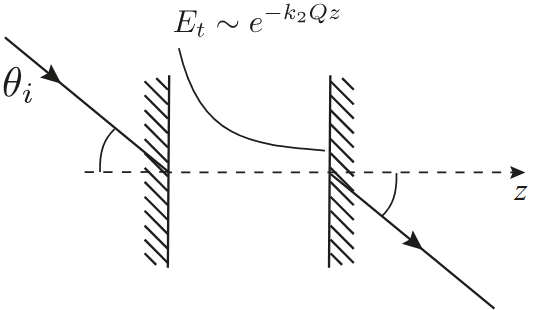
\includegraphics[width=0.5\textwidth]{frustrated.png}
	\caption{}
	\label{fig:frustrated}
\end{figure}
If a wave is travelling in a materials such that it goes dense $\to$ rare $\to$ dense, as in figure \ref{fig:frustrated}. For a thin enough rare material, the evanescent wave can propagate through to the second dense material.

\chapter{Polarisation}
\section{States of Polarisation}

We can resolve any plane polarised wave into its orthogonal components,
\begin{align}
	\vb{E_x} = \vu{i}E_{0_x}\cos(\omega t - kz) && && \vb{E_y} = \vu{j}E_{0_y}\cos(\omega t - kz + \Delta \phi) \\
	&& \vb{E}(z,t) = \vb{E}_x (z,t) + \vb{E}_y(z,t) && 
\end{align}
From this we will base different types of polarisations.
\subsection{Linear Polarisation}
We have 2 forms of linear polarisation,
\begin{itemize}
	\item If $\Delta \phi = \pm2m\pi, m \in \mathbb{Z}$, the components are said to be "in phase".
	\begin{equation}
		\vb{E}(z,t) = (\vu{i}E_{0_x} + \vu{j}E_{0_y})\cos(\omega t - kz)
	\end{equation}
	\item If $\Delta \phi = \pm m\phi$, the components are said to be $180^{\text{o}}$ out of phase.
		\begin{equation}
		\vb{E}(z,t) = (\vu{i}E_{0_x} - \vu{j}E_{0_y})\cos(\omega t - kz)
	\end{equation}
\end{itemize}
\subsection{Circular Polarisation}
Consider $E_0 = E_{0_y} = E_{0_x}$,
\begin{itemize}
	\item If $\Delta \phi = -\frac{\pi}{2} + 2m\pi$, the wave is said to be right circularly polarised, and the wave rotates counter clockwise (looking at the source),
	\begin{equation}
		\vb{E}(z,t) = E_0(\vu{i}\cos(\omega t - kz) + \vu{j}\sin(\omega t - kz)).
	\end{equation}
	\item If $\Delta \phi = \frac{\pi}{2} + 2m\pi$, the light is said to be left circularly polarised, and the wave rotates clockwise,
	\begin{equation}
		\vb{E}(z,t) = E_0(\vu{i}\cos(\omega t - kz) - \vu{j}\sin(\omega t - kz)).
	\end{equation}
\end{itemize}
In the case of $E_{0_x} \neq E_{0_y}$, the light is elliptically polarised.
\section{Mechanisms of Polarisation}
The intensity of a wave is given by,
\begin{equation}
	I = \langle S \rangle = \frac{1}{2}\varepsilon_0 cE^2.
\end{equation}
For randomly polarised light with original intensity $I(\theta)$ and an intensity post-polarisation $I(\theta)$ where $\theta$ is the angle between the transmission axis, the relationship between the two intensities are given by \textit{Malus's law},
\begin{equation}
	I(\theta) = I(0)\cos^2\theta.
\end{equation}
Below we talk about different mechanisms of polarisation.
\subsection{Polarisation by Reflection}
We have previously seen that light incident at the Brewster angle produces light which is completely $S$-polarised.
\subsection{Polarisation by Scattering}
Scattering is when electromagnetic waves incident upon bound electrons set them into vibration with respect to the nucleus. The oscillating electric dipole will then reradiate energy with a frequency coinciding to that of the incident light.
\\\\
If linearly polarised light is incident on a molecule, the direction of the scattered radiation and the oscillating dipole will be coplanar. The dipole will not radiate in the direction of its axis.
\\\\
If randomly polarised light is incident on the molecule, the following will be observed,
\begin{itemize}
	\item The forward direction will be completely unpolarised.
	\item Off-axis radiation will be slightly polarised, and become more polarised as the angle increases.
	\item The direction of observation normal to the incoming light is completely linearly polarised. 
\end{itemize}
\subsection{Polarisation by Dichroism}
This mechanism works by selectively absorbing 1 component of randomly polarised light.
\begin{itemize}
	\item Consists of a material with long, aligned molecules.
	\item Component of the $\vb{E}$ vector along the long axis excites molecules and gets absorbed.
	\item Polarisation of the wave is then along the other axis.
	\item The transmitted field component is $E_0\cos\theta$ where $\theta$ is the angle between the \textit{pass axis}.
\end{itemize}
\section{Optical Anistropy}
We will now talk about materials which are \textit{anistropic} or \textit{birefringent}. We have previously assumed our materials to be isotropic, i.e., that their electric permittivity is the same everywhere. We will no longer be assuming this. When we have an anistropic medium, it results in observing a "double refraction", two shifted images as opposed to just a single image when viewing an object through a medium.
\\\\
The reason we observe anistropy in materials is because in a medium, we have bound electrons which are bound by different amounts in different directions, i.e., there is an anistropy in the binding force. This physical anistropy causes an optical anistropy due to light being absorbed by different amounts in different directions.
\subsection{Modifications to electromagnetic description}
We can construct a wave equation for the electric field in a medium,
\begin{equation}
	-k^2\vb{E} + \vb{k}\left(\vb{k}\cdot\vb{E}\right) = \epsilon\mu \pdv[2]{\vb{E}}{t}.
\end{equation}
We will assume that $\mu = \mu_0$, and since $\epsilon$ has a directional dependence, we will write it as a tensor,
\begin{equation}
	\epsilon = \begin{pmatrix}
		\epsilon_x & 0 & 0 \\
		0 & \epsilon_y & 0 \\
		0 & 0 & \epsilon_z
	\end{pmatrix}
\end{equation}
where we say $\epsilon_x = \epsilon_y \neq \epsilon_z$ for a uniaxial medium, and $\epsilon_x \neq \epsilon_y \neq \epsilon_z$ for a biaxial medium. We can then write out the individual components of $\vb{E}$,
\begin{align}
	-k^2\vb{E} + k_x(\vb{k}\cdot\vb{E}) &= - \epsilon_x\mu \omega^2E_x\\
	-k^2\vb{E} + k_y(\vb{k}\cdot\vb{E}) &= - \epsilon_y\mu \omega^2E_y\\
	-k^2\vb{E} + k_z(\vb{k}\cdot\vb{E}) &= - \epsilon_z\mu \omega^2E_x\\
\end{align}
if we assume $\mu\epsilon_x = \mu\epsilon_y = \frac{n_0^2}{c^2}$ and $\mu\epsilon_z = \frac{n_e^2}{c^2}$, we can solve this system of equations as an eigenvalue equation to obtain,
\begin{equation}
	\boxed{\frac{k^2}{n_0^2} = \frac{\omega^2}{c}}
\end{equation}
\begin{equation}
	\boxed{\frac{k_x^2}{n_e^2} + \frac{k_y^2}{n_e^2} + \frac{k_z^2}{n_o^2} = \frac{\omega^2}{c^2}}
\end{equation}
where we have two refractive indices, the ordinary refractive index $n_0$ and the extraordinary refractive index $n_e$. If we rewrite $k$ space in polar coordinates, we can write down an effective refractive index of the extraordinary wave,
\begin{equation}
	\boxed{\frac{1}{n^2} = \frac{\sin^2\theta}{n_e^2} + \frac{\cos^2\theta}{n_ol^2}}.
\end{equation}
\subsubsection{What is going on here?}
Due to the physical anistropy of anistropic crystals, the molecules within are easier to polarise in some directions over others. This results in the crystal having two different refractive indices - one for light with the $\vb{E}$ vector along the optical axis (extraordinary) and one for light in all other directions (ordinary).
\begin{figure}
	\centering
	\begin{subfigure}{0.4\textwidth}
	\begin{tikzpicture}
		\draw[->] (0,0,0) -- (0,0,5) node[anchor=west] {$z$};
		\draw[->] (0,0,0) -- (2.5,0,0) node[anchor=west] {$x$};
		\draw[->] (0,0,0) -- (0,2.5,0) node[anchor=west] {$y$};
		\draw[latex-latex, very thick] (0, -1, 2.5) -- (0, 1, 2.5) node[anchor=west] {$\vb{E}$};
	\end{tikzpicture}
	\caption{Wave propagating along OA.}
	\end{subfigure}
	\begin{subfigure}{0.4\textwidth}
	\begin{tikzpicture}
		\draw[->] (0,0,0) -- (0,0,5) node[anchor=west] {$z$};
		\draw[->] (0,0,0) -- (2.5,0,0) node[anchor=west] {$x$};
		\draw[->] (0,0,0) -- (0,2.5,0) node[anchor=west] {$y$};
		\draw[latex-latex, very thick] (0, -1, 2.5) -- (0, 1, 2.5) node[anchor=west] {$\vb{E}$};
	\end{tikzpicture}
	\caption{Wave propagating perpendicular to OA.}
	\end{subfigure}
	\caption{}
\end{figure}
\noindent
Let us now consider linearly polarised waves along certain axes. For linearly polarised light propagating different relative to the optical axis.
\begin{enumerate}
	\item \textbf{Propagating Along Optic Axis}
	\begin{itemize}
		\item The $\vb{E}$ vectors are in the $xy$ plane. 
		\item $\vb{E}$ oscillates perpendicular to the optical axis.
		\item All polarisation components of the wave experience $n_o$.
		\item There is no change in polarisation, the wave travels at $v = \frac{c}{n_o}$.
	\end{itemize}
	\item \textbf{Propagating $\perp$ to Optic Axis - Polarised $\perp$ to Optic Axis}
	\begin{itemize}
		\item Components all experience $n_o$.
		\item There is no change in polarisation.
		\item The wave travels at  $v = \frac{c}{n_o}$.
	\end{itemize}
	\item \textbf{Propagating $\perp$ to Optic Axis - Polarised $\parallel$ to Optic Axis}
	\begin{itemize}
		\item Components all experience $n_e$.
		\item There is no change in polarisation.
		\item The wave travels at  $v = \frac{c}{n_e}$.
	\end{itemize}
	\item \textbf{Polarised at $45^{\text{o}}$ to Optic Axis}
	\begin{itemize}
		\item $x$ component $\parallel$ to optic axis $\implies$ travels at $\frac{c}{n_e}$.
		\item $y$ component $\perp$ to optic axis $\implies$ travels at $\frac{c}{n_o}$.
		\item $x$ and $y$ components are out of phase.
	\end{itemize}
	\item \textbf{Arbitrarily Polarised Wave} (see fig. \ref{fig:eo})
	\begin{itemize}
		\item Some components are $\parallel$ to optical axis, some are $\perp$.
		\item The wave front is elliptically polarised when striking the crystal. 
		\item Components $\perp$ to optical axis will travel at $\frac{c}{n_o}$.
		\begin{itemize}
			\item These known as \textit{o-rays} - wave proceeds without deviation and wavefronts are circular.
		\end{itemize}
		\item Components $\parallel$ to the optical axis and travel at a higher speed $\frac{c}{n_0}$.
		\begin{itemize}
			\item These are known as \textit{e-rays} - wave fronts are elliptical, direction of propagation is no longer perpendicular to wavefront. 
		\end{itemize}
	\end{itemize}
\end{enumerate}
\begin{figure}
	\centering
	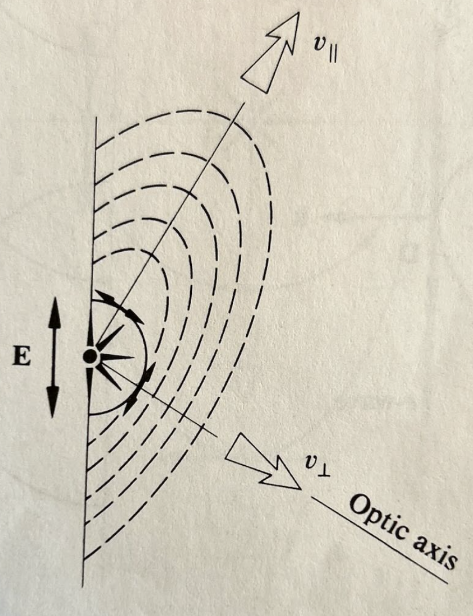
\includegraphics[width=0.4\textwidth]{eo.png}
	\caption{}
	\label{fig:eo}
\end{figure}
\subsection{Retardation Plates}
Retardation plates are objects which take advantage of $e$ waves travelling faster than $o$ waves, causing a phase shift between the two. They will cause an optical path difference given by,
\begin{equation}
	p = \abs{d(n_0 - n_e)}
\end{equation}
where $d$ is the travel distance.
\subsubsection{Quarter Wave Plates}
Quarter wave plates cause a path difference,
\begin{equation}
	d(n_0 - n_e) = \frac{\lambda}{4}.
\end{equation}
Considering an input wave,
\begin{equation}
	E_0\vu{x}\cos(\omega t - kz) + E_0\vu{y}\cos(\omega t - kz)
\end{equation}
we can see that this wall cause a phase shift of $\frac{\pi}{2}$, i.e., the output wave will be,
\begin{equation}
	E_0\vu{x}\cos\left(\omega t - kz + \frac{\pi}{2}\right) + E_0\vu{y}\cos(\omega t - kz)
\end{equation}
thus the output wave will be circularly polarised.
\subsubsection{Half Wave Plate}
A half wave plate causes,
\begin{equation}
	d(n_0 - n_e) = \frac{\lambda}{2}.
\end{equation}
and thus a phase difference of $\pi$, so the input and output waves are,
\begin{align}
	\text{Input} && E_0\vu{x}\cos(\omega t - kz) + E_0\vu{y}\cos(\omega t - kz) \\
	\text{Output} && -E_0\vu{x}\cos(\omega t - kz) + E_0\vu{y}\cos(\omega t - kz)
\end{align}
thus the wave is still linearly polarised, but the polarisation angle is flipped about the optic axis. This is such that the input wave makes an angle $\arctan\left(\frac{E_{0_y}}{E_{0_x}}\right)$ with the optic axis, and the output wave makes an angle $-\arctan\left(\frac{E_{0_y}}{E_{0_x}}\right)$ with the optic axis.
\chapter{Interference}
Interference comes from adding waves. I.e., if we have 2 waves $\vb{E}_1$ and $\vb{E}_2$, the interference wave $\vb{E}$ would be,
\begin{equation}
	\vb{E} = \vb{E}_{1_0} e^{i(\omega_1 -\vb{k}_1\cdot{\vb{r}} + \varepsilon_1)} + \vb{E}_{2_0} e^{i(\omega_2 -\vb{k}_2\cdot{\vb{r}} + \varepsilon_2)}.
\end{equation}
To get the intensity pattern we would have to calculate $\vb{E}^*\vb{E}$. However, this is cumbersome. Instead, we can use \textit{phasors}. If we consider $\vb{E}_1$ and $\vb{E}_2$ as connected lines in the complex plane at an angle $\omega_1 -\vb{k}_1\cdot{\vb{r}} + \varepsilon_1$ and $ \omega_2 -\vb{k}_2\cdot{\vb{r}} + \varepsilon_2$ to the $x$-axis, we can simply apply simple geometry and the cosine rule,
\begin{equation}
	I = \abs{\vb{E}}^2 = E_{1_0}^2 + E_{2_0}^2 + 2E_{1_0}E_{2_0}\cos((\omega_1 - \omega_2)t -(\vb{k}_1 - \vb{k}_2)\cdot\vb{r} + (\varepsilon_1 - \varepsilon_2))
\end{equation}
\section{Coherence}
For waves to interfere, they much be coherent. They must satisfy the following conditions,
\begin{enumerate}
	\item \textit{Temporal Coherence} - $\omega_1 \simeq \omega_2$.
	\item \textit{Spatial Coherence} - $\varepsilon_1 - \varepsilon_2$ must be constant over time.
\end{enumerate}
\subsection{Temporal Coherence}
This is a measure of the average correlation of the phase of the wave along the direction of propagation. We define a \textit{coherence time},
\begin{equation}
	\tau_c = \frac{1}{\Delta \mu}
\end{equation}
which is the time frame that the wave oscillates over a predicable time, and $\Delta \mu$ is the spectral width of the light source. The longer the coherence time, the greater the temporal coherence of the source. We can calculate the corresponding coherence length,
\begin{equation}
	\Delta x_c = c\tau_c
\end{equation}
which is the distance over which the wave visibly spreads out.
\subsection{Spatial Coherence}
Spatial coherence is the correlation of the phase of a light wave transverse to the propagation direction. The range of separation, $\Delta x$ between two points over which there is significant interference defines the coherence area $A_c$. 
\section{Division of Wavefronts}
If a wave encounters a barrier that has an opening similar to its wavelength, it will diffract. 
\subsection{Young's Double Slit}
\begin{figure}[h]
	\centering 
	\begin{subfigure}{0.4\textwidth}
		\centering
		\begin{tikzpicture}
			
			\def\L{5.9}       % distance between walls
			\def\H{3.0}       % total wall height
			\def\f{0.9}       % fractional height of projection point
			\def\ang{atan((\f*\H+\a)/\L/2)} % theta
			\def\t{0.15}      % wall thickness
			\def\a{1.5}       % slit distance
			\def\d{0.20}      % slit size
			\coordinate (T) at (0,\a/2);
			\coordinate (B) at (0,-\a/2);
			\coordinate (L) at (0,0);
			\coordinate (R) at (\L,0);
			\coordinate (P) at (\L,\f*\H/2);
			\coordinate (M) at ($(B)!(T)!(P)$);
			
			% LINES
			\draw[mygreen,thick] (T) -- (P) node[midway,above=-1] {$r_1$};
			\draw[mygreen,thick] (B) -- (P) node[midway,below=3,right=6] {$r_2$}; %right=6,below right=-4
			\draw[dashed] (L) -- (P);
			\draw[dashed,black!60] (L) -- (R);
			\draw[mydarkred,dashed] (M) -- (T);
			
			% ANGLES
			\draw pic[mysmallarr,"$\theta'$",mydarkred,draw=mydarkred,angle radius=26,angle eccentricity=1.25]
			{angle = B--T--M};
			\draw pic[mysmallarr,"$\theta$",mydarkred,draw=mydarkred,angle radius=38,angle eccentricity=1.14]
			{angle = R--L--P};
			\rightAngle{T}{M}{P}{0.3}
			
			% MEASURES
			\draw[<->,black] (0,-0.47*\H) --++ (\L,0) node[midway,fill=white,inner sep=1] {$D >> d$};
			\draw[<->,black] (-2.1*\t,-\a/2) --++ (0,\a) node[midway,fill=white,inner sep=1] {$d$};
			\draw[<->,black] ([shift={({\ang-90}:0.1)}]B) -- ([shift={({\ang-90}:0.1)}]M)
			node[midway,above=1,below right=-3]{$d\sin\theta'$};
			\draw[<->,black] ([shift={(2.1*\t,0)}]P) -- ([shift={(2.1*\t,0)}]R)
			node[midway,fill=white,inner sep=1]{$y$};
			
			% WALL
			\fill[wall]
			(0,\a/2-\d/2) rectangle (-\t,-\a/2+\d/2)
			(0,\a/2+\d/2) rectangle (-\t,\H/2)
			(0,-\a/2-\d/2) rectangle (-\t,-\H/2)
			(\L,-\H/2) rectangle (\L+\t,\H/2);
			\fill[mygreen!80!black] (P) circle (0.3*\t) node[right=1,above left=-2] {P};
			
		\end{tikzpicture}
		\caption{}
	\end{subfigure}
	\begin{subfigure}{0.4\textwidth}
		\centering
		% TWO SLIT PATH DIFFERENCE close up
		\begin{tikzpicture}
			
			\def\L{5.5}       % distance between walls
			\def\l{3.8}       % distance between walls
			\def\H{3.5}       % total wall height
			\def\f{0.9}       % fractional height of projection point
			\def\t{0.15}      % wall thickness
			\def\a{1.6}       % slit distance
			\def\d{0.20}      % slit size
			\def\ang{27}      % angle
			\coordinate (T) at (0,\a/2);
			\coordinate (B) at (0,-\a/2);
			\coordinate (L) at (0,0);
			\coordinate (R) at (\L,0);
			\coordinate (I) at ({\a/2/tan(\ang)},0);
			
			% LINES
			\draw[mygreen,thick] (T) --++ (\ang:.8*\l) coordinate (PT) node[midway,below=1,above left=-2] {$r_1$};
			\draw[mygreen,thick] (B) --++ (\ang:\l) coordinate (PB) node[midway,left=2,below right=-1] {$r_2$};
			\draw[mydarkred,dashed] (T) -- ($(B)!(T)!(PB)$) coordinate (M);
			\draw[black!60,dashed] (L) --++ (\ang:.9*\l) coordinate (PR);
			%\draw[black!60,dashed] (T) --++ (.20*\L,0) coordinate (TR);
			\draw[black!60,dashed] (L) --++ (.6*\L,0) coordinate (LR);
			%\draw[black!60,dashed] (B) --++ (.20*\L,0) coordinate (BR);
			
			% LINE END
			\lineend{PT}{\ang+70}
			\lineend{PB}{\ang+70}
			
			% ANGLES
			\draw pic[mysmallarr,"\contour{white}{$\theta$}",mydarkred,draw=mydarkred,angle radius=18.8,angle eccentricity=1.38 ]
			{angle = B--T--M};
			%\draw pic[->,"$\theta$",mydarkred,draw=mydarkred,angle radius=16,angle eccentricity=1.41]
			%  {angle = TR--T--PT};
			%\draw pic[->,"$\theta$",mydarkred,draw=mydarkred,angle radius=16,angle eccentricity=1.41]
			%  {angle = BR--B--PB};
			\draw pic[mysmallarr,"$\theta$",mydarkred,draw=mydarkred,angle radius=22,angle eccentricity=1.25]
			{angle = LR--L--PR};
			\draw pic[mysmallarr,"$\theta$",mydarkred,draw=mydarkred,angle radius=22,angle eccentricity=1.30]
			{angle = LR--I--PB};
			\rightAngle{T}{M}{PB}{0.3}
			
			% MEASURES
			\draw[<->,black] (-2.2*\t,-\a/2) --++ (0,\a) node[midway,fill=white,inner sep=1.5] {$d$};
			\draw[<->,black] ([shift={({\ang-90}:0.1)}]B) -- ([shift={({\ang-90}:0.1)}]M)
			node[midway,above=1,below right=-3]{$\Delta L$};
			
			% WALL
			\fill[wall]
			(0,\a/2-\d/2) rectangle (-\t,-\a/2+\d/2)
			(0,\a/2+\d/2) rectangle (-\t,\H/2)
			(0,-\a/2-\d/2) rectangle (-\t,-\H/2);
			
		\end{tikzpicture}
		\caption{}
	\end{subfigure}
	\caption{}
\end{figure}
In Young's double slit, we make the following assumptions,
\begin{itemize}
	\item $D >> d$
	\item $\omega_1 = \omega_2$, $k_1 = k_2$, $\varepsilon_1 - \varepsilon_2 = d\sin\theta$.
	\item Ignore $\vb{r}$ dependence on $\vb{E}$.
	\item Interfering waves are parallel and apart by $d\cos\theta$.
\end{itemize}
If we recall our formulation for adding the intensity of two waves, we find,
\begin{equation}
	\begin{split}
		I(y) & = 2E^2(1+\cos(kd\sin\theta)) \\
		& =  4E^2\left(\cos^2\left(\frac{kd\sin\theta}{2}\right)\right) = 4E^2\cos^2\left(\frac{kdy}{2D}\right) = 4E^2\cos^2\frac{\pi dy}{\lambda D}.
	\end{split}
\end{equation}
We then clearly see that we obtain bright fringes at,
\begin{align}
	\frac{kdy}{2D} = n\pi && \frac{dy}{\lambda D} = n && d\sin\theta = n\lambda
\end{align}
which is true for two slits.
\begin{tcolorbox}[title={Visbility of fringe patterns}, width=\textwidth]
	The visibility of fringe patterns is given by,
	\begin{equation}
		V = \frac{I_{\text{max}} - I_{\text{min}}}{I_{\text{max}} + I_{\text{min}}}
	\end{equation}
	which is $V = 1$ for Young's experiment because $I_{\text{min}} = 0$. However, this is not always the case, particularly for the case of $n$ slits.
\end{tcolorbox}
\subsection{Lloyd's Mirror}
\begin{figure}[h]
	\centering
	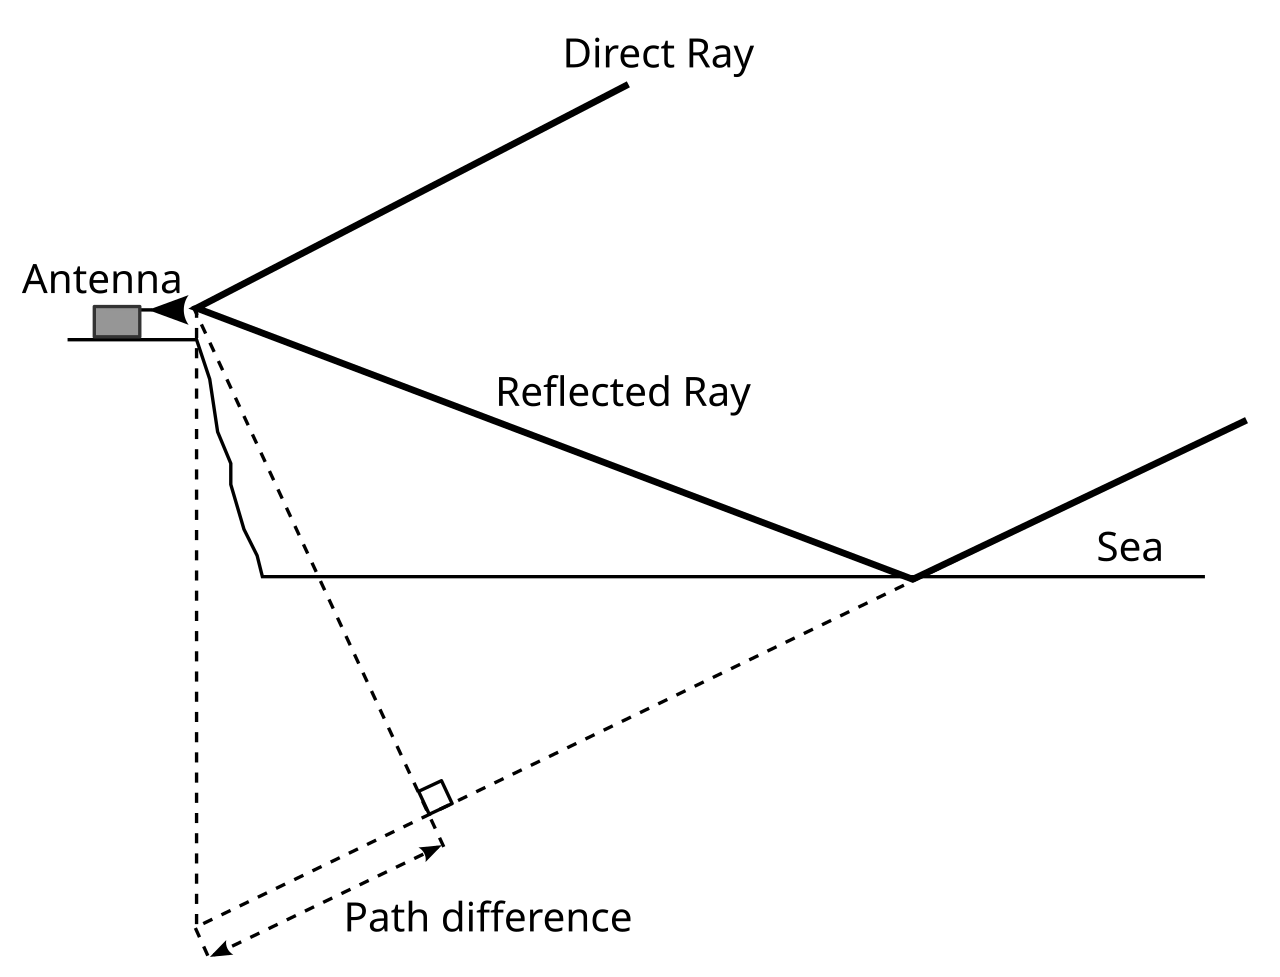
\includegraphics[width=0.45\textwidth]{lloyd.png}
	\caption{}
\end{figure}
Lloyd's mirror produces identical effects to Young's double slit experiment, but relies on the reflection of a single source in order to produce two coherent waves. This reflection causes a phase shift of $\pi$. From Young's slit,
\begin{equation}
	\begin{split}
		I(y) & = 4E^2\cos^2\left(\frac{kd\sin\theta}{2}\pm \frac{\pi}{2}\right) \\
		& = 4E^2\sin^2\left(\frac{kd\sin\theta}{2}\right)
	\end{split}
\end{equation}
thus the difference we see is that dark fringes occur at $n\pi$. 
\subsection{Three and $n$ slits}
We can extend Young's double slit into 3 fringes. Without proof, the summation of 3 of the electric waves is,
\begin{equation}
	E_{\text{tot}} = E(1+2\cos(kd\sin\theta))
\end{equation}
and the intensity is,
\begin{equation}
	I(y) = E^2\left(4\cos^2\left(\frac{kd\sin\theta}{2} - 1\right)\right)^2
\end{equation}
and we find that there is a splitting in the fringes, with a single diminished fringe in between. 
\\\\
We can extend this to $n$ fringes by,
\begin{equation}
	I(y) = |E_0|^2\frac{\sin^2\left(\frac{Nk\delta}{2}\right)}{\sin^2\left(\frac{k\delta}{2}\right)}.
\end{equation}
\section{Amplitude Splitting Interferometers}
\begin{figure}[h]
	\centering
	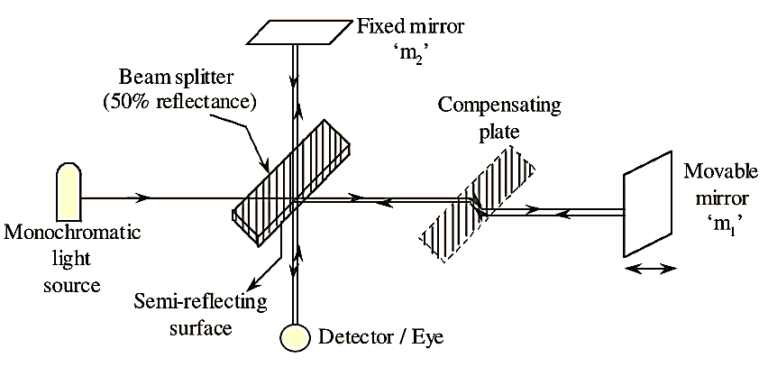
\includegraphics[width=0.5\textwidth]{interferometer.png}
	\caption{}
	\label{fig:interferometer}
\end{figure}\noindent
We can also obtain interference by the division of amplitudes. We can achieve this by the use of an interferometer, as in figure \ref{fig:interferometer}. If the vertical distance between the mirrors is $d_1$, and the horizontal distance between the mirrors is $d_2$, then the path difference of the light as it hits the detector is,
\begin{equation}
	\Delta = 2(d_1 - d_2).
\end{equation}
As the light hits the enters the splitter, it reflects on a rare-dense interface, so picks up a $\pi$ phase difference. Thus, the intensity pattern is given by,
\begin{equation}
	I(y) = 4|E|^2\sin^2\left(\frac{\pi\Delta}{\lambda}\right)
\end{equation}
so, we have dark fringes at $\Delta = m \lambda$, and bright fringes at $\Delta = m\lambda/2$ of intensity $I = 4|E|^2$. As we change the position of the mirrors, we see shifts in the dark and bright rings. 
\subsection{Fringe Formation}
\begin{figure}[h]
	\centering
	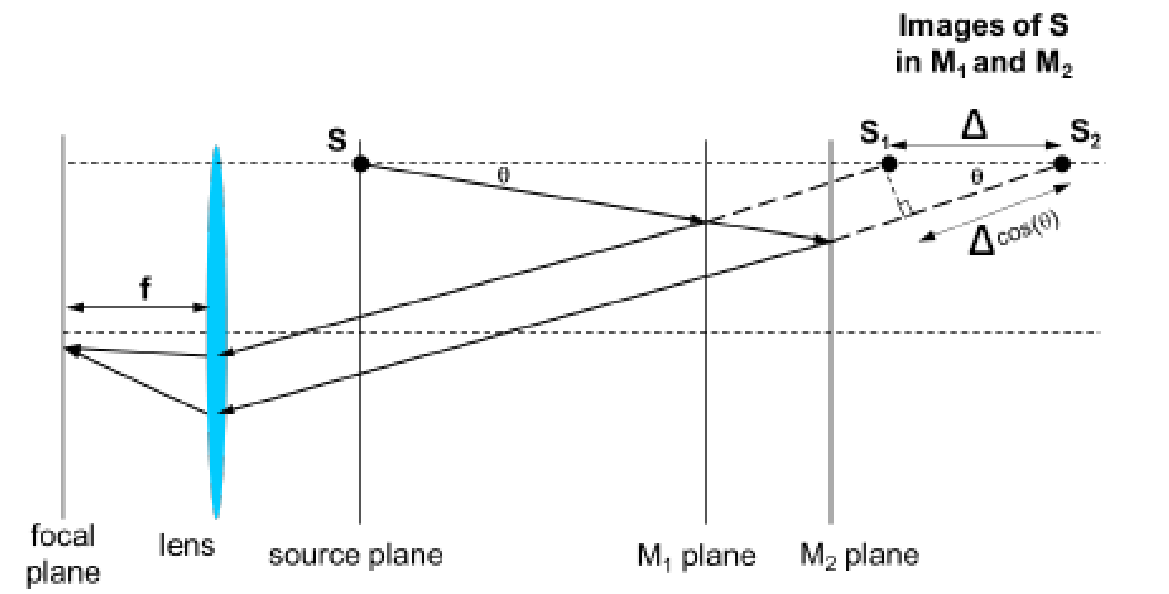
\includegraphics[width=0.6\textwidth]{fringe.png}
	\caption{}
	\label{fig:fringe}
\end{figure}\noindent
Let us now consider the formation of fringes due to geometric optics considerations, as in figure \ref{fig:fringe}. We observe dark fringes at $2(d_1 - d_2)\cos\theta = m\lambda$, and we observe the $p$th dark fringe at,
\begin{equation}
	2(d_1 - d_2)\cos\theta = (m-p)\lambda
\end{equation} 
thus, we observe a central dark fringe at $\theta = 0$, $2(d_1 - d_2) = m\lambda$. The angular position of any ring is,
\begin{equation}
	\begin{split}
	2(d_1 - d_2)\cos\theta & = m\lambda - p\lambda \\
	& = 2(d_1 - d_2) - p\lambda
	\end{split}
\end{equation}
so,
\begin{equation}
	p\lambda = 2(d_1 - d_2)(1-cos\theta) 
\end{equation}
and applying the small angle approximation,
\begin{equation}
	\theta = \left(\frac{p\lambda}{d_1 - d_2}\right)^{1/2}
\end{equation}
which is the angular radius of the $p$th ring, which we can write as,
\begin{equation}
	\theta^2 = \frac{2p\lambda}{\Delta}
\end{equation}
\subsection{Thin Film Interference}
\begin{figure}[h]
	\centering
	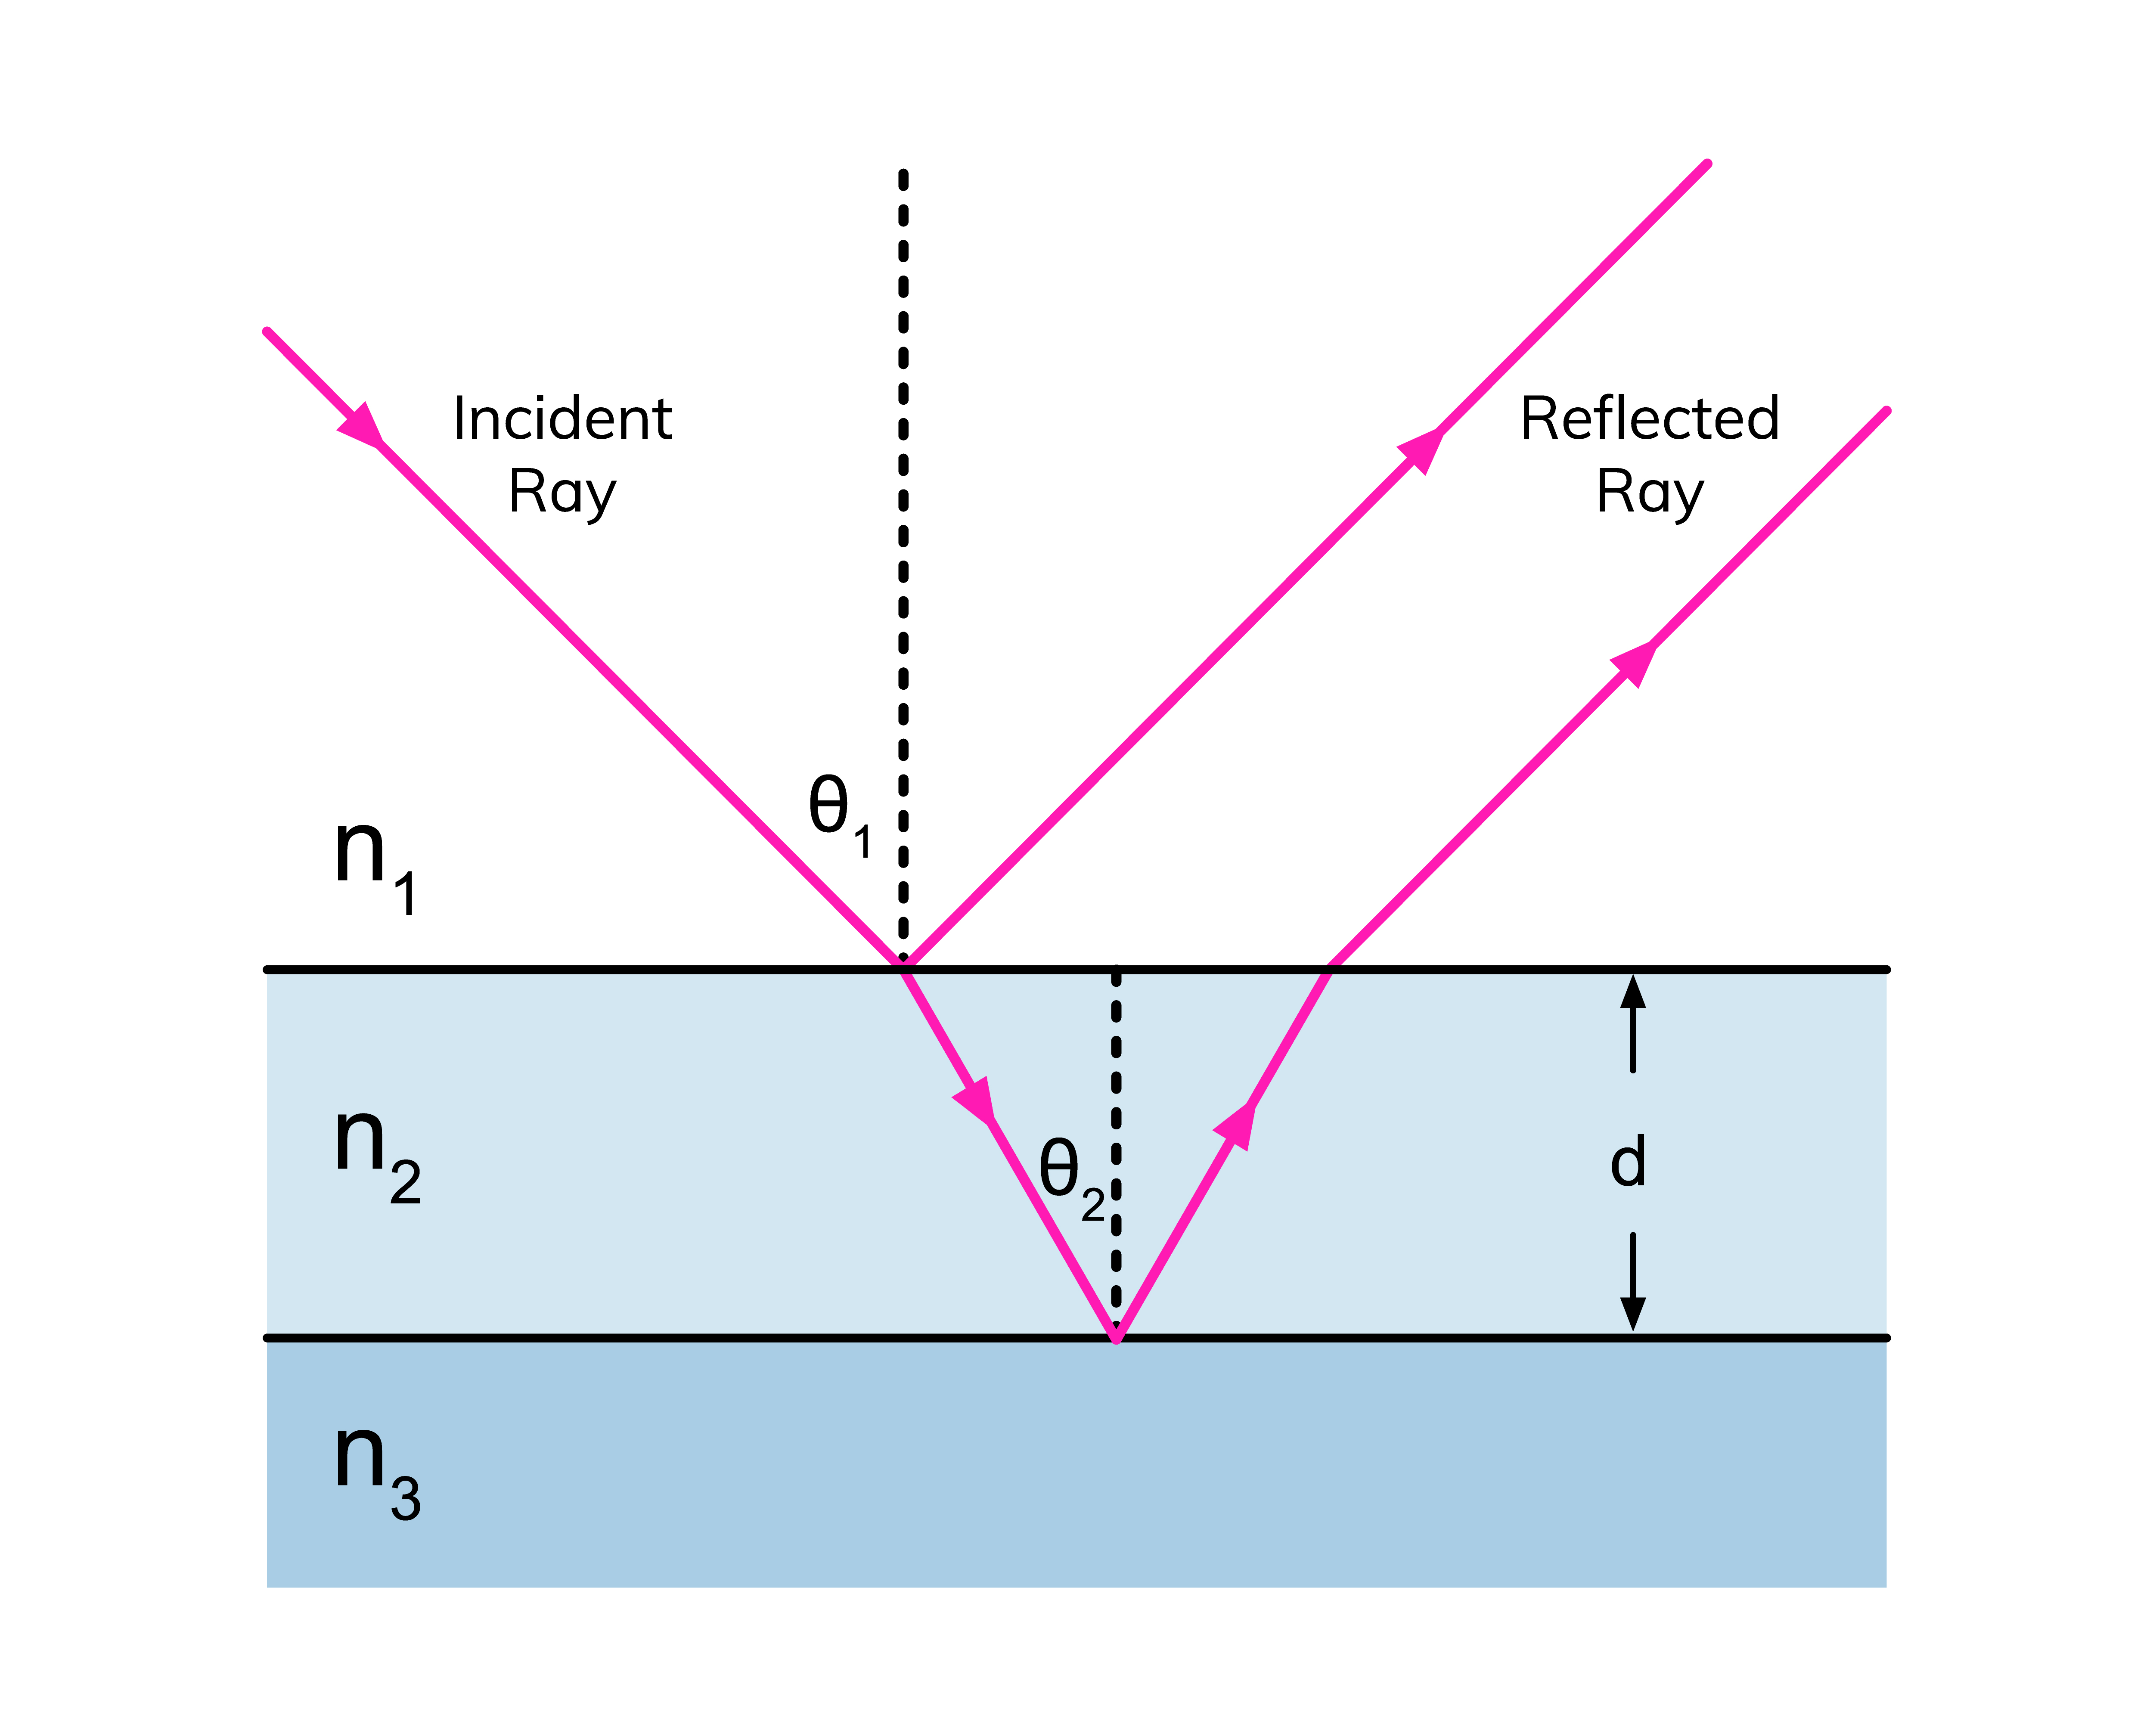
\includegraphics[width=0.6\textwidth]{thinfilm.jpg}
	\caption{}
	\label{fig:thin film}
\end{figure}
Thin film interference occurs when light enters a material and then totally internally refracts back through where it came from, as in figure \ref{fig:thin film}. For a film of thickness $d$ and refractive index $n$, the path difference is given by,
\begin{equation}
	\begin{split}
		\Delta & = \frac{2dn}{\cos\theta_r} - 2d\tan\theta_r\sin\theta_i \\
			& = \frac{2dn}{\cos\theta_r} - 2d\tan\theta_rn\sin\theta_r
	\end{split}
\end{equation}
where $\theta_i$ is the angle of incidence onto the film and $\theta_r$ is the angle of reflection within the film. Applying appropriate identities, 
\begin{equation}
	\Delta = 2d\left(\frac{n-n\sin^2\theta_r}{\cos\theta_r}\right) = \boxed{2dn\cos\theta_r},
\end{equation}
The typical result we would expect is for $\Delta \propto \sin\theta_r$, so we see that the reflection within the thin film adds a $\pi$ phase difference. 
\subsection{Fabry-Perot Etalon}
\begin{figure}
	\centering
	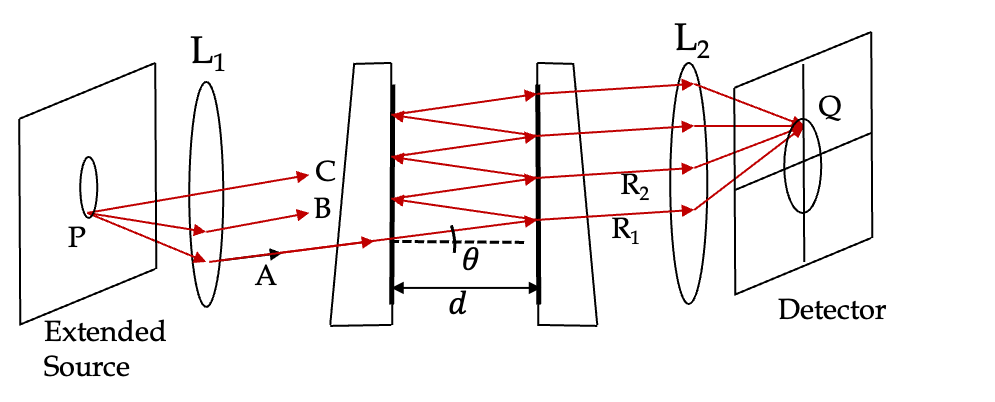
\includegraphics[width=0.6\textwidth]{fabry-perot-interferometer-setup.png}
	\caption{}
	\label{fig:fabryperot}
\end{figure}
A Fabry-Perot Etalon is shown in figure \ref{fig:fabryperot}. It consists of two, perfectly parallel plates with a highly reflective, semi-transparent coating with reflection coefficient $\rho$ and transmission coefficient $\sigma$. The distance between the plates $d$ is small and fixed. The apparatus is very sensitive to optical path difference, and each successive within the interferometer is weaker than the last by $\sqrt{\rho}^2$. Each wave has a phase shift of
\begin{equation}
	\delta = \frac{2\pi}{\lambda}\cdot2d\cos\theta
\end{equation}
with respect to the last. 
\subsubsection{Intensity Distribution}
Given the phase shift of each wave, the wave is given by,
\begin{equation}
	E_{\text{tot}} = E_0e^{i(kz-\omega t)}(\sigma + \sigma\rho e^{i\delta} + \sigma \rho^2e^{2i\delta} + \cdots) 
\end{equation}
which we can rewrite
\begin{equation}
	E_{\text{tot}} = E_0\sigma e^{i(kz - \omega t)}\frac{1}{1-\rho e^{i\delta}}
\end{equation}
by inspection, considering the expansion of $(1-x)^{-1}$. Forming $I = E_{\text{tot}}^*E_{\text{tot}}$ as usual, we find,
\begin{equation}
	I = \frac{E_0^2\sigma^2}{1 + \rho^2 + 2\rho\cos\delta}
\end{equation}
which we can rearrange to form,
\begin{equation}
	I(\delta) = \frac{E_0^2\sigma^2}{(1-\rho)^2\left(1+\frac{4\rho}{(1-\rho^2)}\sin^2(\delta/2)\right)}.
\end{equation}
\begin{figure}[h]
	\centering
	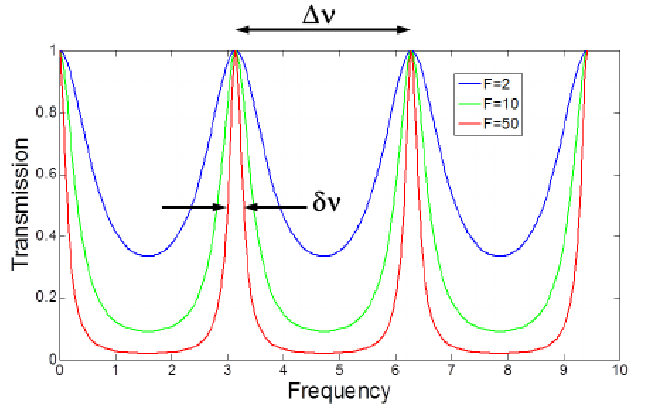
\includegraphics[width=0.5\textwidth]{fab.png}
	\caption{}
	\label{fig:fab}
\end{figure}
Let us analyse the intensity pattern, plotted in figure \ref{fig:fab}. We find sharp peaks where,
\begin{equation}
	\delta = \frac{2\pi}{\lambda}2d\cos\theta = 2\pi m.
\end{equation}
$\delta \lambda$ is the resolution, given by,
\begin{equation}
	\delta \lambda = \frac{\lambda(1- \rho)}{\pi m \sqrt{\rho}}
\end{equation}
and $\Delta \lambda$ is the spectral range. The ratio of these two quantities is known as the finesse,
\begin{equation}
	\frac{\Delta \lambda}{\delta \lambda} = \frac{\pi \sqrt{\rho}}{1 - \rho}
\end{equation}
and is a measure of how sharp the peaks are. 
\chapter{Diffraction}
The Fourier transform is defined,
\begin{equation}
	\mathcal{F}\left\{f(x)\right\} = F(k) = \int_{-\infty}^{\infty}f(x)e^{-ikx}\dd{x}
\end{equation}
The Fourier transform of the functional representation of ga slit allows us to obtain the diffraction pattern produced when light enters through the slit. Common Fourier transforms are,
\begin{itemize}
	\item Top hat $\rightarrow$ $\text{sinc}$
	\item Gaussian $\leftrightarrow$ Gaussian
	\item Constant $\to$ $\delta(x)$
	\item $\delta(x + x_0) + \delta(x - x_0)$ $\to$ $2\cos(k\frac{x_0}{2})$.
\end{itemize} 
We will also be using convolution in order to simplify some diffraction problems. Convolution is the act of "smearing" two functions together. It is defined,
\begin{equation}
	h(x) = f(x) * g(x) = \int_{-\infty}^{\infty}f(x')g(x-x')\dd{x'}.
\end{equation}
We can imagine convolution as sliding a function $f$ over $g$, and the convolution being the accumulation of their mutual area as we slide over each function.
\\\\
We will be making use of the convolution theorem, which states that, if $h$ is a convolution of $f$ and $g$, then
\begin{equation}
	\mathcal{F}\left\{h\right\} = \mathcal{F}\left\{f\right\}\cdot\mathcal{F}\left\{g\right\}.
\end{equation}
\section{Fraunhofer (Far Field) Diffraction}
\subsection{Fraunhofer Diffraction From a Single Slit}
\begin{figure}[h]
	\centering
	\begin{tikzpicture}
		\message{Diffraction, path difference (close-up)^^J}
		
		\def\L{6.15}      % distance between walls
		\def\l{4.0}       % path length
		\def\H{4.3}       % total wall height
		\def\f{0.9}       % fractional height of projection point
		\def\t{0.15}      % wall thickness
		\def\a{2.5}       % slit distance
		\def\ang{26}      % angle
		\coordinate (T) at (0,\a/2);
		\coordinate (B) at (0,-\a/2);
		\coordinate (L) at (0,0);
		\coordinate (R) at (\L,0);
		\coordinate (I) at ({\a/2/tan(\ang)},0);
		
		% LINES
		\draw[mygreen,thick] (T) --++ (\ang:.8*\l) coordinate (PT); %node[midway,below=1,above left=-2] {$r_1$};
		\draw[mygreen,thick] (B) --++ (\ang:\l) coordinate (PB); %node[midway,left=2,below right=-1] {$r_2$};
		\draw[mygreen,thick] (L) --++ (\ang:.9*\l) coordinate (PR);
		\draw[dashed] (T) -- (B);
		\draw[mydarkred,dashed] (T) -- ($(L)!(T)!(PR)$) coordinate (M);
		%\draw[black!60,dashed] (T) --++ (.20*\L,0) coordinate (TR);
		\draw[black!60,dashed] (L) --++ (.6*\L,0) coordinate (LR);
		%\draw[black!60,dashed] (B) --++ (.20*\L,0) coordinate (BR);
		
		% LINE END
		\lineend{PT}{\ang+70}
		\lineend{PR}{\ang+70}
		\lineend{PB}{\ang+70}
		
		% ANGLES
		\draw pic[mysmallarr,"$\theta$",mydarkred,draw=mydarkred,angle radius=20,angle eccentricity=1.3]
		{angle = B--T--M}; %\contour{white}{}
		\draw pic[mysmallarr,"$\theta$",mydarkred,draw=mydarkred,angle radius=24,angle eccentricity=1.2]
		{angle = LR--L--PR};
		\draw pic[mysmallarr,"$\theta$",mydarkred,draw=mydarkred,angle radius=24,angle eccentricity=1.2]
		{angle = LR--I--PB};
		\rightAngle{T}{M}{PR}{0.3}
		
		% MEASURES
		\draw[<->,black] (-2.1*\t,0) --++ (0,\a/2) node[midway,fill=white,inner sep=0.1] {$a/2$};
		\draw[<->,black] (-2.1*\t,0) --++ (0,-\a/2) node[midway,fill=white,inner sep=0.1] {$a/2$};
		\draw[<->,black] ([shift={({\ang-90}:0.1)}]L) -- ([shift={({\ang-90}:0.1)}]M)
		node[midway,left=5,below right=-1]{$\frac{a}{2}\!\sin\theta$};
		
		% WALL
		\fill[wall]
		(0,\a/2) rectangle (-\t,\H/2)
		(0,-\a/2) rectangle (-\t,-\H/2);
		
	\end{tikzpicture}
	\caption{}
	\label{fig:fraun}
\end{figure}
Fraunhofer diffraction from a single slit is shown in figure \ref{fig:fraun}. We will assume as the wave passes through the slit, that each infinitesimal amplitude is equal. We will also assume that the pattern is seen at a large distance. can be modelled as a top-hat function, i.e.,
\begin{equation}
	f(x) = \begin{cases}
		1 & -\frac{a}{2} < x < \frac{a}{2}\\
		0 & \text{Otherwise}.
	\end{cases}
\end{equation}
If we take the Fourier transform of a top hat, we obtain the $\text{sinc}$ function. The intensity will be given by,
\begin{equation}
	I = E_0^2\text{sinc}^2\left(\frac{a\pi \sin\theta}{\lambda}\right).
\end{equation}
\subsection{Fraunhofer From Two Slits}
We must take advantage of the convolution theorem. For this, we want to convolve 2 delta functions, separated by a distance $d$, with a top hat function of width $a$. This results in an intensity pattern of,
\begin{equation}
	I \propto \cos^2\left(\frac{\pi d \sin\theta}{\lambda}\right)\text{sinc}^2\left(\frac{\pi a \sin\theta}{\lambda}\right).
\end{equation}
\section{Huygens-Fresnel Integral}
\begin{figure}[h]
	\centering
	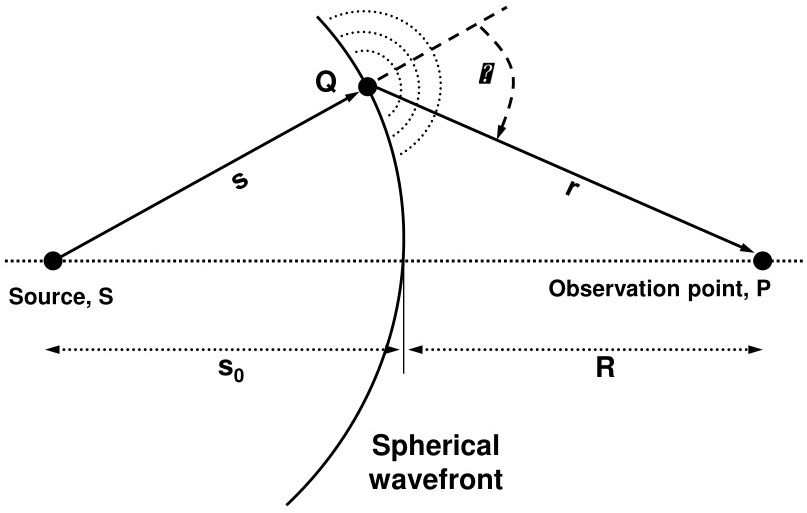
\includegraphics[width=0.5\textwidth]{huygens.jpg}
	\caption{}
	\label{fig:huygens}
\end{figure}\noindent
All points on a wavefront can be considered as a point source for the production of secondary, spherical wave fronts. Let us consider figure \ref{fig:huygens}. The wave at $Q$ is given by,
\begin{equation}
	E(Q) \propto \frac{e^{iks}}{s}
\end{equation}
where the wave is radiated towards $P$, and is modified by,
\begin{equation}
	K(\alpha) = \frac{1}{2}\left(1 + \cos\alpha\right).
\end{equation}
At $P$, 
\begin{equation}
	\dd{E} = K(\alpha) \epsilon'\frac{e^{iks}}{s}\frac{e^{ikr}}{r}\dd{A}
\end{equation}
and the Huygens-Fresnel integral is given by,
\begin{equation}
	\boxed{E(P) = \epsilon'\frac{e^{iks}}{s}\int K(\alpha) \frac{e^{ikr}}{r}\dd{A}}
\end{equation}
where $\dd{A}$ is an integral over the aperture.
\section{Fresnel Diffraction}
\begin{figure}
	\centering
	\begin{tikzpicture}
		\def\myshift#1{\raisebox{1ex}}
		\draw (0,5) -- (0,4);
		\draw (0,0) -- (0,1);
		\draw (1,5.1) arc (170:190:15);
		\draw (0,5) -- (0.9,4.5) node[midway, above] {\rotatebox{-26.56}{$\delta$}};
		\draw (0.9,4.5) -- (5,2.5) node[midway, above] {\rotatebox{-26.56}{$\sim z$}};
		\node[anchor=west]  at (5,2.5) {$P$};
		\node at (5,2.5) {\textbullet};
		\draw[dashed] (5,2.5) -- (5,0);
		\draw[dashed] (5,2.5) -- (-2,2.5);
		\draw[dashed] (0,5) -- (-2,5);
		\draw[<->] (-1,5) -- (-1,2.5) node[midway, anchor=west] {$y$};
		\draw[<->] (0,-.5) -- (5,-.5) node[midway, anchor=north] {$z$}; 
	\end{tikzpicture}
	\caption{}
	\label{fig:fresnel}
\end{figure}\noindent
In Fresnel diffraction, we no longer assume the source is infinitely far away. We will see that this leads to the phase contribution no longer being linear. Consider figure \ref{fig:fresnel}. If we assume $y << z$, we can calculate,
\begin{equation}
	\begin{split}
	\delta & = \sqrt{y^2 + z^2} - z \\
	& = z \sqrt{1 + \frac{y^2}{z^2}} - z \\
	& \simeq z\left(1 + \frac{y^2}{2z^2}\right) - z = \frac{y^2}{2z^2},
\end{split}
\end{equation}the phase difference,
\begin{equation}
	k\delta = \frac{\pi y^2}{\lambda z}.
\end{equation}
The boundary between Fraunhofer and Fresnel diffraction is known as the Raleigh distance,
\begin{equation}
	z_r = \frac{2y^2}{\lambda}.
\end{equation}
\subsection{Diffraction from Straight Edges and Slits}
\begin{figure}[h]
	\centering
	\begin{tikzpicture}
		\node at (-2,0) {\textbullet};
		\node[anchor=east] at (-2,0) {$S$};
		\node at (0,0) {\textbullet};
		\node at (4,0) {\textbullet};
		\node[anchor=west] at (4,0) {$P$};
		\draw (0,2) -- (0,1);
		\draw (0,-2) -- (0,-1);
		\draw[<->] (-2,0) -- (0, 1) node[midway, above] {\rotatebox{26.56}{$s$}};
		\draw[<->] (0,1) -- (4,0) node[midway,above] {\rotatebox{-14.04}{$r$}};
		\draw[dashed, <->] (-2,0) -- (0,0) node[midway,below] {$S_0$};
		\draw[dashed, <->] (0,0) -- (4,0) node[midway,below] {$R$};
		\node at (4,2) {{\small$x$} $\odot$};
		\draw[->] (4.25,2) -- (4.75,2) node[anchor=west] {\small$z$};
		\draw[->] (4.14, 2.125) -- (4.14,2.625) node[anchor=south] {\small$y$};
	\end{tikzpicture}
	\caption{}
	\label{fig:straightedge}
\end{figure}
Consider figure \ref{fig:straightedge},
\begin{align}
	r^2 & = R^2 + x^2 + y^2 \\
	s^2 & = S_0^2 + x^2 + y^2
\end{align}
so,
\begin{equation}
	\begin{split}
	r + s & = R\left(1 + \frac{x^2 + y^2}{R^2}\right)^{1/2} + S_0\left(1+ \frac{x^2  + y^2}{S_0}\right)^{1/2}\\
	& \simeq R+S_0 + (x^2+y^2)\left(\frac{S_0 + R}{2S_0R}\right)
	\end{split}
\end{equation}
where the latter term in the second line is the path difference. We have,
\begin{equation}
	\frac{S_0 + R}{S_0R} = \frac{1}{R} + \frac{1}{S_0} = \frac{1}{z}
\end{equation}
so the path difference is,
\begin{equation}
	\text{path diff.} = \frac{x^2+y^2}{2z}.
\end{equation}
The electric field will be given by considering the Huygens-Fresnel integral. We will assume $K(\alpha)$ is constant, and $s$ and $r$ are constant in the denominator, but not in phase. So,
\begin{equation}
	\begin{split}
	E(P) &= \frac{\epsilon'K(\alpha)}{S_0R}\int e^{ik(r+s)}\dd{A} \\
	& = \text{constants}\int e^{i\frac{2\pi}{\lambda}\frac{x^2}{2z}}\dd{x}\int e^{i\frac{2\pi}{\lambda}\frac{y^2}{z^2}}\dd{y}.
	\end{split}
\end{equation}
We can now make a substitution,
\begin{align}
	u = x\sqrt{\frac{2}{\lambda z}} && v = y\sqrt{\frac{2}{\lambda z}},
\end{align}
so we now have,
\begin{equation}
	E(P) = \text{constants}\int e^{i\frac{\pi}{2}u^2}\dd{u} \int e^{i\frac{\pi}{2}v^2}\dd{y},
\end{equation}
we want to split this integral into its real and imaginary components,
\begin{align}
	C(\omega) = \int_0^{\omega}\cos\left(\frac{\pi}{2}\omega'^2\right)\dd{\omega'} && S(\omega) = \int_0^{\omega}\sin\left(\frac{\pi}{2}\omega'^2\right)\dd{\omega'}.
\end{align}
The equations above have no analytic solution. We can instead plot them as parametric equations to obtain a \textit{cornu spiral}, as in figure \ref{fig:cornuspiral}. On this graph, $(0,0)$ represents the centre of the aperture. If we find the $\omega$ corresponding to the ends of the aperture, draw a line between them and find the distance between them, it will tell us the magnitude of the resultant electric field.
\begin{figure}
	\centering
	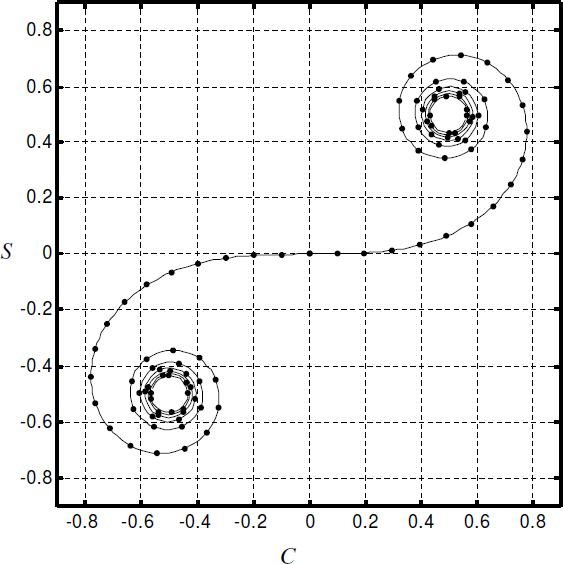
\includegraphics[width=0.5\textwidth]{cornu.PNG}
	\caption{}
	\label{fig:cornuspiral}
\end{figure}
\section{Diffraction Grating}
\begin{figure}[h]
	\centering
	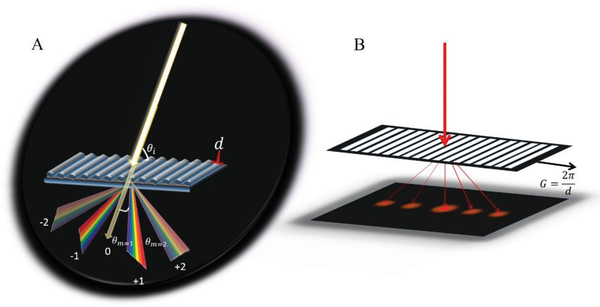
\includegraphics[width=0.5\textwidth]{diff.png}
	\caption{}
	\label{fig:diff}
\end{figure}
A diffraction grating is a repetitive array of diffracting elements, such as apertures or obstacles. This results in periodic alterations in amplitude, phase, or both. Figure \ref{fig:diff} shows the two types of grating.
\subsection{Transmission Phase Grating}
These consist of parallel notches of flat, clear glass. Its grating equation is given by,
\begin{equation}
	d\sin\alpha - d\sin\beta = m\lambda
\end{equation}
where $\alpha$ is the angle of the incoming wave, and $\beta$ is the angle of the outgoing wave.
\subsection{Transmission Amplitude Grating}
If there are $N$ slits separated by $d$ with width $a$, we must convolve $N$ delta functions with a single wise slit, which leads to an intensity pattern,
\begin{equation}
	I \propto \frac{sin^2\left(\frac{Nd\sin\theta \pi}{\lambda}\right)}{\sin^2\left(\frac{d\sin\theta \pi}{\lambda}\right)}\text{sinc}^2\left(\frac{\pi a \sin\theta}{\lambda}\right).
\end{equation}
Furthermore, we will observe the separation of wavelengths. If we have, $d\sin\theta = m\lambda$, we find,
\begin{equation}
	\dv{\theta}{\lambda} = \frac{m}{d\cos\theta}
\end{equation}
which is known as \textit{dispersion}.
\appendix
\chapter{Revision Equations}
\section{Potentials}
\begin{tcolorbox}[colback=red!5!white,colframe=red!75!black,title=Static Electric Potential]
	\begin{align}
		\vb{E} &= - \grad \phi \\
		\laplacian{\phi} &= - \frac{\rho}{\varepsilon_0}
	\end{align}
\end{tcolorbox}
\begin{tcolorbox}[colback=blue!5!white,colframe=blue!75!black,title=Static Magnetic Potential]
	\begin{align}
		\vb{B} &= \curl{\vb{A}} \\
		-\curl{\vb{B}} &= \laplacian{\vb{A}} = - \mu_0 \vb{J}
	\end{align} 
	if we choose,
	\begin{align}
		\vb{A} \to \vb{A} + \grad{\psi} && \div{\vb{A}} = 0.
	\end{align}
\end{tcolorbox}
\begin{tcolorbox}[colback=green!5!white,colframe=green!75!black,title=Dynamic Potentials]
	\begin{align}
		\laplacian\vb{A} - \mu_0\varepsilon_0 \pdv{\vb{A}}{t} &= - \mu_0 \vb{J} \label{eq:A} \\
		\laplacian\vb{\phi} - \mu_0\varepsilon_0\pdv{\phi}{t} &= -\frac{\rho}{\varepsilon_0} \label{eq:phi}
	\end{align}
\end{tcolorbox}
\section{Gauges}
\begin{tcolorbox}[colback=red!5!white,colframe=red!75!black,title=Coloumb Gauge]
	\begin{equation}
		\div{\vb{A}} = 0
	\end{equation}
\end{tcolorbox}
\begin{tcolorbox}[colback=blue!5!white,colframe=blue!75!black,title=Lorenz Gauge]
	\begin{equation}
		\div{\vb{A}} + \frac{1}{c^2}\pdv{\phi}{t} = 0
	\end{equation}
\end{tcolorbox}
\section{Vector Identities}
\begin{tcolorbox}[colback=blue!5!white,colframe=blue!75!black,title=Laplacian of a Vector]
	\begin{equation}
		\curl{\curl{\vb{A}}} = \grad\left(\div{\vb{A}}\right) - \laplacian{\vb{A}}
	\end{equation}
\end{tcolorbox}
\section{EM Waves}
\begin{tcolorbox}[colback=red!5!white,colframe=red!75!black,title=Relation between $\vb{E}$ and $\vb{B}$]
	\begin{equation}
		\vb{B} = \frac{1}{c}\hat{\vb{k}}\cross \vb{E}. \label{eq:A4}
	\end{equation}
\end{tcolorbox}

\end{document}
